%%%%%%%%%%%%%%%%%%%%%%%%%%%%%%%%%%%%%%%%%
% Manual (Documentation Template)
% LaTeX Template
% Version 1.0 (05/01/2018)
%
% This template has been downloaded from:
% http://www.LaTeXTemplates.com
%
% Original author:
% Francisco Maria Calisto
%
% License:
% Apache License (Version 2.0)
%
% IMPORTANT NOTE:
% In addition to running BibTeX to compile the
% reference list from the .bib
% file, you will need to run MakeIndex to compile
% the index at the end of the document.
%
%%%%%%%%%%%%%%%%%%%%%%%%%%%%%%%%%%%%%%%%%

%--------------------------------------------------
%	PACKAGES AND OTHER DOCUMENT CONFIGURATIONS
%--------------------------------------------------

\documentclass{tufte-book} % Use the tufte-book class which in turn uses the tufte-common class

\usepackage{graphicx}
\graphicspath{ {graphics/} }

% encoding
%--------------------------------------
\usepackage[utf8]{inputenc}
\usepackage[T1]{fontenc}
%--------------------------------------
 
% Portuguese-specific commands
%--------------------------------------
\usepackage[english]{babel}
%--------------------------------------

% Uncomment this line if you prefer colored hyperlinks
% (e.g., for onscreen viewing)
%--------------------------------------
\hypersetup{colorlinks}
%--------------------------------------

%%
% Book metadata
\title{User Manual\\(EN)}
\author[User Manual]{ISR \& INESC-ID}
\publisher{MIMBCD-UI}

%%
% If they're installed, use Bergamo and Chantilly from www.fontsite.com.
% They're clones of Bembo and Gill Sans, respectively.
%\IfFileExists{bergamo.sty}{\usepackage[osf]{bergamo}}{}% Bembo
%\IfFileExists{chantill.sty}{\usepackage{chantill}}{}% Gill Sans

%\usepackage{microtype}

%%
% Just some sample text
\usepackage{lipsum}

%%
% For nicely typeset tabular material
\usepackage{booktabs}

%%
% For graphics / images
\usepackage{graphicx}
\setkeys{Gin}{width=\linewidth,totalheight=\textheight,keepaspectratio}
\graphicspath{{graphics/}}

% The fancyvrb package lets us customize the formatting of verbatim
% environments.  We use a slightly smaller font.
\usepackage{fancyvrb}
\fvset{fontsize=\normalsize}

%%
% Prints argument within hanging parentheses (i.e., parentheses that take
% up no horizontal space).  Useful in tabular environments.
\newcommand{\hangp}[1]{\makebox[0pt][r]{(}#1\makebox[0pt][l]{)}}

%%
% Prints an asterisk that takes up no horizontal space.
% Useful in tabular environments.
\newcommand{\hangstar}{\makebox[0pt][l]{*}}

%%
% Prints a trailing space in a smart way.
\usepackage{xspace}

%%
% Some shortcuts for Tufte's book titles.  The lowercase commands will
% produce the initials of the book title in italics.  The all-caps commands
% will print out the full title of the book in italics.
\newcommand{\vdqi}{\textit{VDQI}\xspace}
\newcommand{\ei}{\textit{EI}\xspace}
\newcommand{\ve}{\textit{VE}\xspace}
\newcommand{\be}{\textit{BE}\xspace}
\newcommand{\VDQI}{\textit{The Visual Display of Quantitative Information}\xspace}
\newcommand{\EI}{\textit{Envisioning Information}\xspace}
\newcommand{\VE}{\textit{Visual Explanations}\xspace}
\newcommand{\BE}{\textit{Beautiful Evidence}\xspace}

\newcommand{\TL}{Tufte-\LaTeX\xspace}

% Prints the month name (e.g., January) and the year (e.g., 2008)
\newcommand{\monthyear}{%
  \ifcase\month\or January\or February\or March\or April\or May\or June\or
  July\or August\or September\or October\or November\or
  December\fi\space\number\year
}


% Prints an epigraph and speaker in sans serif, all-caps type.
\newcommand{\openepigraph}[2]{%
  %\sffamily\fontsize{14}{16}\selectfont
  \begin{fullwidth}
  \sffamily\large
  \begin{doublespace}
  \noindent\allcaps{#1}\\% epigraph
  \noindent\allcaps{#2}% author
  \end{doublespace}
  \end{fullwidth}
}

% Inserts a blank page
\newcommand{\blankpage}{\newpage\hbox{}\thispagestyle{empty}\newpage}

\usepackage{units}

% Typesets the font size, leading, and measure in the form of 10/12x26 pc.
\newcommand{\measure}[3]{#1/#2$\times$\unit[#3]{pc}}

% Macros for typesetting the documentation
\newcommand{\hlred}[1]{\textcolor{Maroon}{#1}}% prints in red
\newcommand{\hangleft}[1]{\makebox[0pt][r]{#1}}
\newcommand{\hairsp}{\hspace{1pt}}% hair space
\newcommand{\hquad}{\hskip0.5em\relax}% half quad space
\newcommand{\TODO}{\textcolor{red}{\bf TODO!}\xspace}
\newcommand{\ie}{\textit{i.\hairsp{}e.}\xspace}
\newcommand{\eg}{\textit{e.\hairsp{}g.}\xspace}
\newcommand{\na}{\quad--}% used in tables for N/A cells
\providecommand{\XeLaTeX}{X\lower.5ex\hbox{\kern-0.15em\reflectbox{E}}\kern-0.1em\LaTeX}
\newcommand{\tXeLaTeX}{\XeLaTeX\index{XeLaTeX@\protect\XeLaTeX}}
% \index{\texttt{\textbackslash xyz}@\hangleft{\texttt{\textbackslash}}\texttt{xyz}}
\newcommand{\tuftebs}{\symbol{'134}}% a backslash in tt type in OT1/T1
\newcommand{\doccmdnoindex}[2][]{\texttt{\tuftebs#2}}% command name -- adds backslash automatically (and doesn't add cmd to the index)
\newcommand{\doccmddef}[2][]{%
  \hlred{\texttt{\tuftebs#2}}\label{cmd:#2}%
  \ifthenelse{\isempty{#1}}%
    {% add the command to the index
      \index{#2 command@\protect\hangleft{\texttt{\tuftebs}}\texttt{#2}}% command name
    }%
    {% add the command and package to the index
      \index{#2 command@\protect\hangleft{\texttt{\tuftebs}}\texttt{#2} (\texttt{#1} package)}% command name
      \index{#1 package@\texttt{#1} package}\index{packages!#1@\texttt{#1}}% package name
    }%
}% command name -- adds backslash automatically
\newcommand{\doccmd}[2][]{%
  \texttt{\tuftebs#2}%
  \ifthenelse{\isempty{#1}}%
    {% add the command to the index
      \index{#2 command@\protect\hangleft{\texttt{\tuftebs}}\texttt{#2}}% command name
    }%
    {% add the command and package to the index
      \index{#2 command@\protect\hangleft{\texttt{\tuftebs}}\texttt{#2} (\texttt{#1} package)}% command name
      \index{#1 package@\texttt{#1} package}\index{packages!#1@\texttt{#1}}% package name
    }%
}% command name -- adds backslash automatically
\newcommand{\docopt}[1]{\ensuremath{\langle}\textrm{\textit{#1}}\ensuremath{\rangle}}% optional command argument
\newcommand{\docarg}[1]{\textrm{\textit{#1}}}% (required) command argument
\newenvironment{docspec}{\begin{quotation}\ttfamily\parskip0pt\parindent0pt\ignorespaces}{\end{quotation}}% command specification environment
\newcommand{\docenv}[1]{\texttt{#1}\index{#1 environment@\texttt{#1} environment}\index{environments!#1@\texttt{#1}}}% environment name
\newcommand{\docenvdef}[1]{\hlred{\texttt{#1}}\label{env:#1}\index{#1 environment@\texttt{#1} environment}\index{environments!#1@\texttt{#1}}}% environment name
\newcommand{\docpkg}[1]{\texttt{#1}\index{#1 package@\texttt{#1} package}\index{packages!#1@\texttt{#1}}}% package name
\newcommand{\doccls}[1]{\texttt{#1}}% document class name
\newcommand{\docclsopt}[1]{\texttt{#1}\index{#1 class option@\texttt{#1} class option}\index{class options!#1@\texttt{#1}}}% document class option name
\newcommand{\docclsoptdef}[1]{\hlred{\texttt{#1}}\label{clsopt:#1}\index{#1 class option@\texttt{#1} class option}\index{class options!#1@\texttt{#1}}}% document class option name defined
\newcommand{\docmsg}[2]{\bigskip\begin{fullwidth}\noindent\ttfamily#1\end{fullwidth}\medskip\par\noindent#2}
\newcommand{\docfilehook}[2]{\texttt{#1}\index{file hooks!#2}\index{#1@\texttt{#1}}}
\newcommand{\doccounter}[1]{\texttt{#1}\index{#1 counter@\texttt{#1} counter}}

% Generates the index
\usepackage{makeidx}
\makeindex

\begin{document}

% r.3 full title page
\maketitle

\let\cleardoublepage\clearpage

% r.5 contents
\tableofcontents

\let\cleardoublepage\clearpage

% r.9 Introduction
\chapter{Intro}

Your decision to use the MIMBCD-UI Cornerstone Prototype shows your commitment to total practice of medical imaging diagnosis for a multimodality view. MIMBCD-UI Project can help you visualize all of your patient’s modalities, not only, for the breast cancer diagnosis, but also, for other medical and educational information purpose.

\hfill

\textbf{Why MIMBCD-UI System?}

\hfill

MIMBCD-UI tool offers you:

\begin{itemize}
\item \textbf{Flexibility}~\textendash~MIMBCD-UI Cornerstone Prototype is an Open Source project where you can add functionality as you want;
\item \textbf{Functionality}~\textendash~You can add functionality from the Cornerstone Library;
\item \textbf{Help}~\textendash~You can quickly look up information and get answers to questions using the Help system built into MIMBCD-UI Cornerstone Prototype or by reading documentation;
\item \textbf{Multimodality}~\textendash~You can work in more than one image modality at the same time;
\item \textbf{Sharing}~\textendash~You can share the information with other users;
\item \textbf{Simplicity}~\textendash~MIMBCD-UI Cornerstone Prototype is easy to learn and easy to use;
\item \textbf{Support}~\textendash~Open Source community to supports you;
\end{itemize}

\hfill

A browser application used to only view projection radiographs (e.g. US or MRI) could be designed around using a mouse with a mouse wheel.

\hfill

\begin{center}
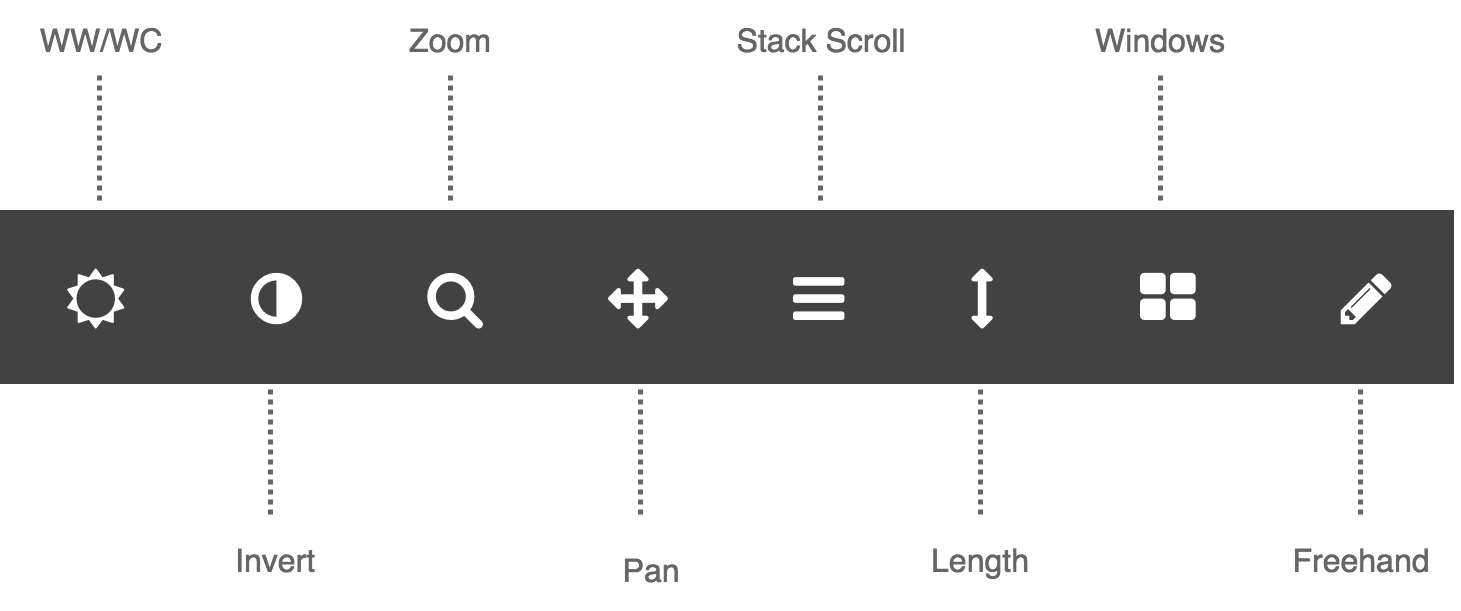
\includegraphics[width=\textwidth]{graphics/tools.png}
\end{center}

\hfill

The functionality exposed would are as follows:

\hfill

\begin{enumerate}
\item Change Luminosity (\textbf{WW/WC});
\item \textbf{Invert};
\item \textbf{Zoom} In and \textbf{Zoom} Out;
\item Image Position (\textbf{Pan});
\item \textbf{Stack Scroll};
\item \textbf{Length} Measurement;
\item Manage Number of \textbf{Windows};
\item Annotations (\textbf{Freehand});
\end{enumerate}

\hfill

The mouse wheel would be used to \textbf{Zoom} the image. The UI would present a button for the other tools allowing the user to select which one to use the LEFT mouse button for. For example, the user could press the \textbf{WW/WC} button and the adjust the \textbf{WW/WC} by LEFT click dragging. After this, they could select the \textbf{Length} button and left click drag to create a length measurement.

% r.10 Study List
\chapter{Study List}

In this section we will describe the Study List, or more vulgarly known as list of patients. Study List allows to visualize your studies and patients.

\hfill

\begin{center}
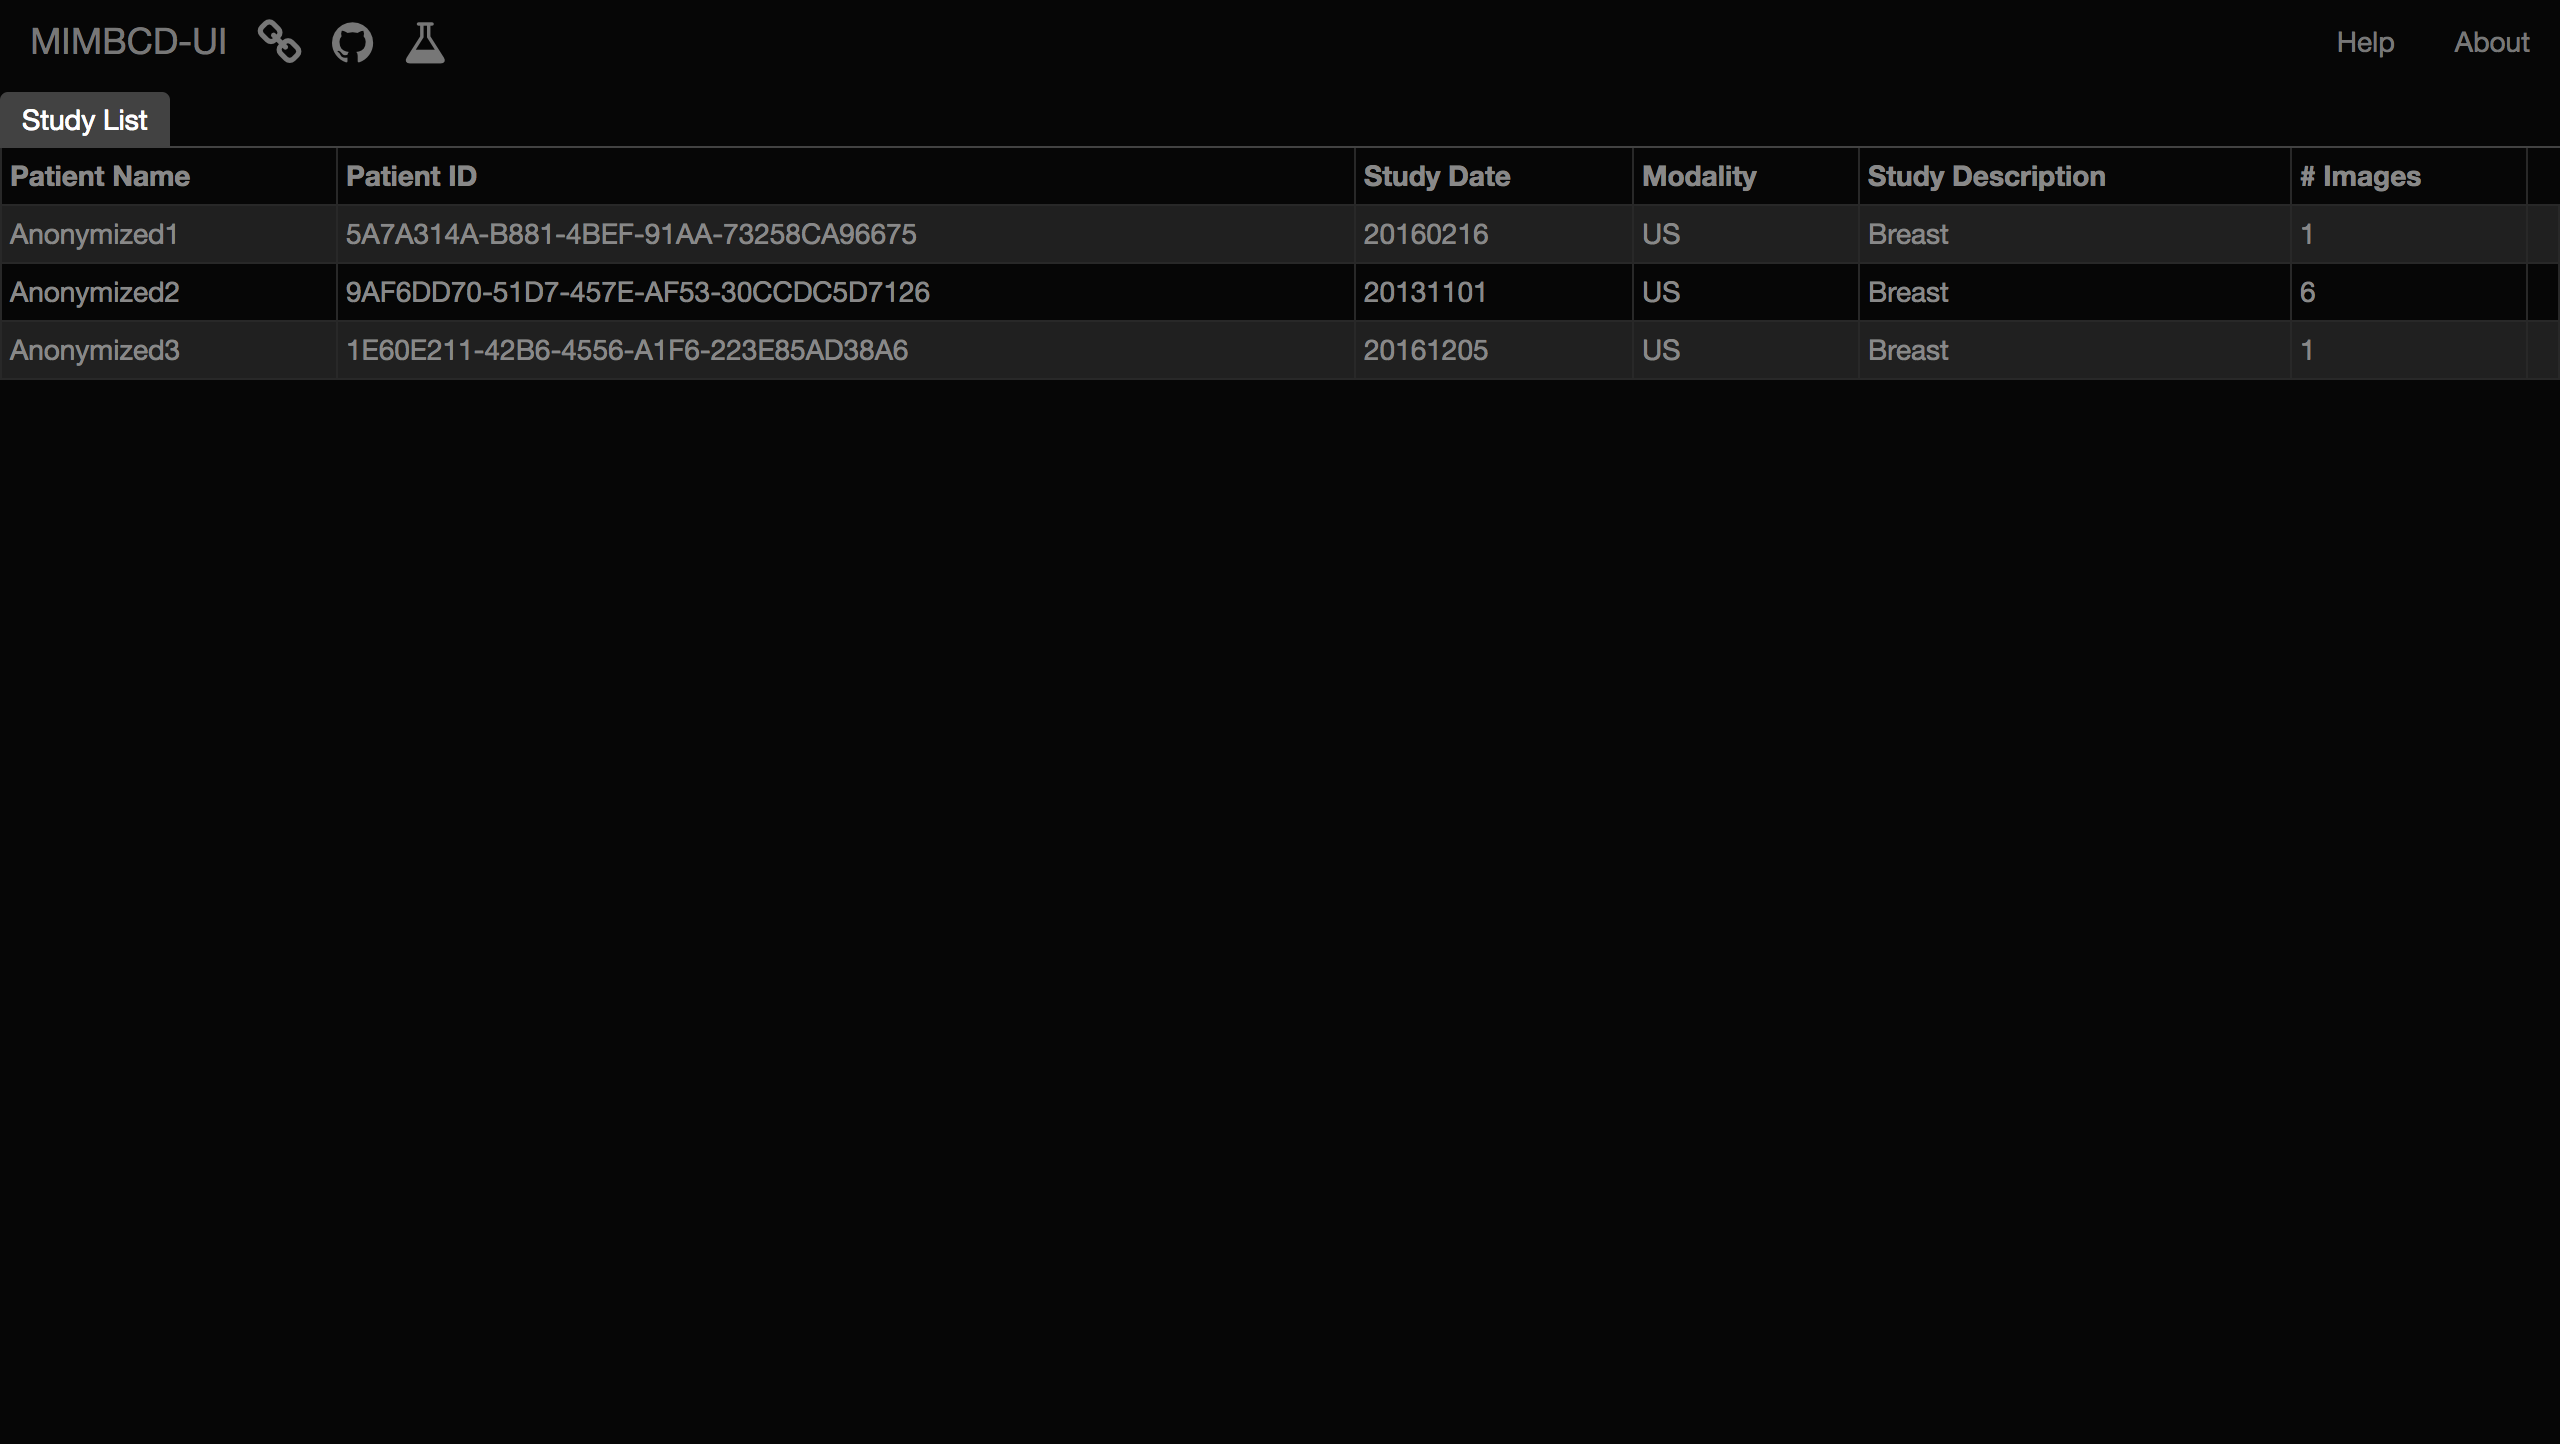
\includegraphics[width=\textwidth]{graphics/study_list_base.png}
\end{center}

\hfill

\clearpage

\hfill

\begin{enumerate}
\item Open the MIMBCD-UI Cornerstone Prototype;
\item Each column has the following description:
\begin{enumerate}
\item \textbf{Patient Name}~\textendash~The name of the patient linked from your PACS;
\item \textbf{Patient ID}~\textendash~ The ID of the patient;
\item \textbf{Study Date}~\textendash~The date when the study was created or edited;
\item \textbf{Modality}~\textendash~Modality of the image or the set of modalities of the patient;
\item \textbf{Study Description}~\textendash~Description of the study;
\item \textbf{Images}~\textendash~Number of images of the patient;
\end{enumerate}
\item By pressing with the patient with LEFT mouse button, you will open the study;
\end{enumerate}

\hfill

\begin{center}
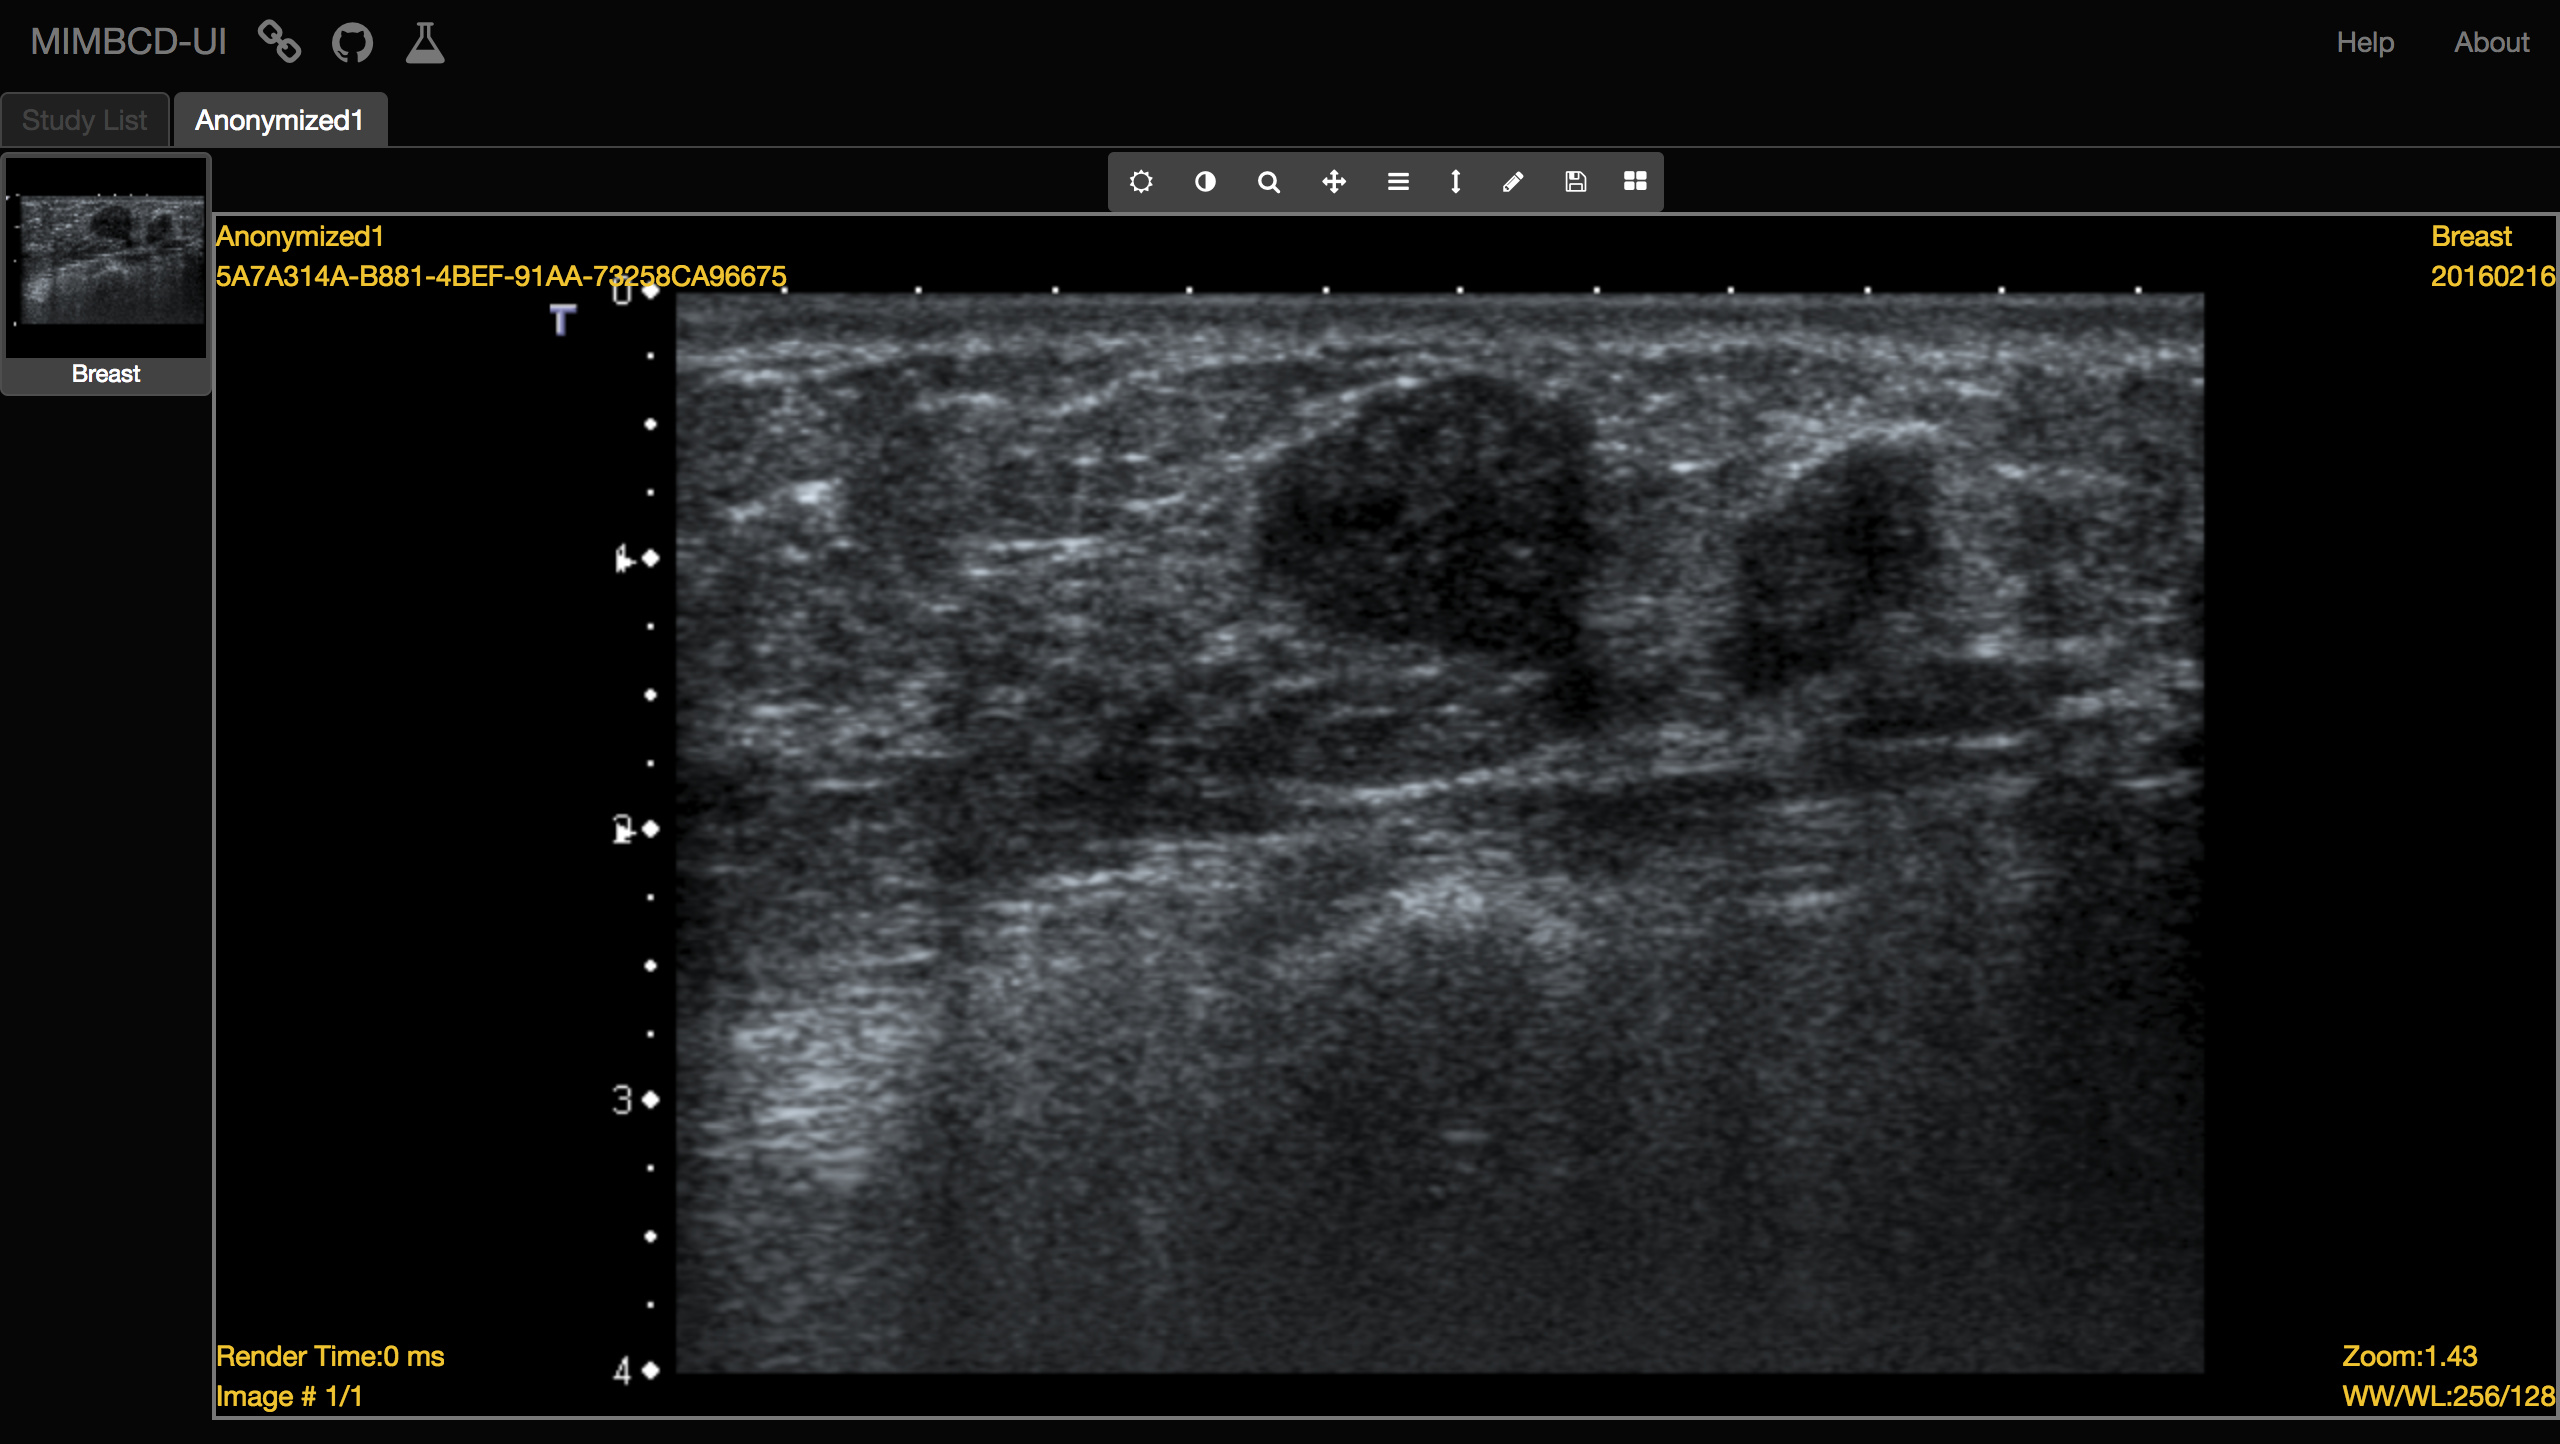
\includegraphics[width=\textwidth]{graphics/anon1_open.png}
\end{center}

\hfill

% r.11 WW/WC
\chapter{WW/WC}

\begin{enumerate}

\item Select the \textbf{WW/WC} option;

\hfill

\begin{center}
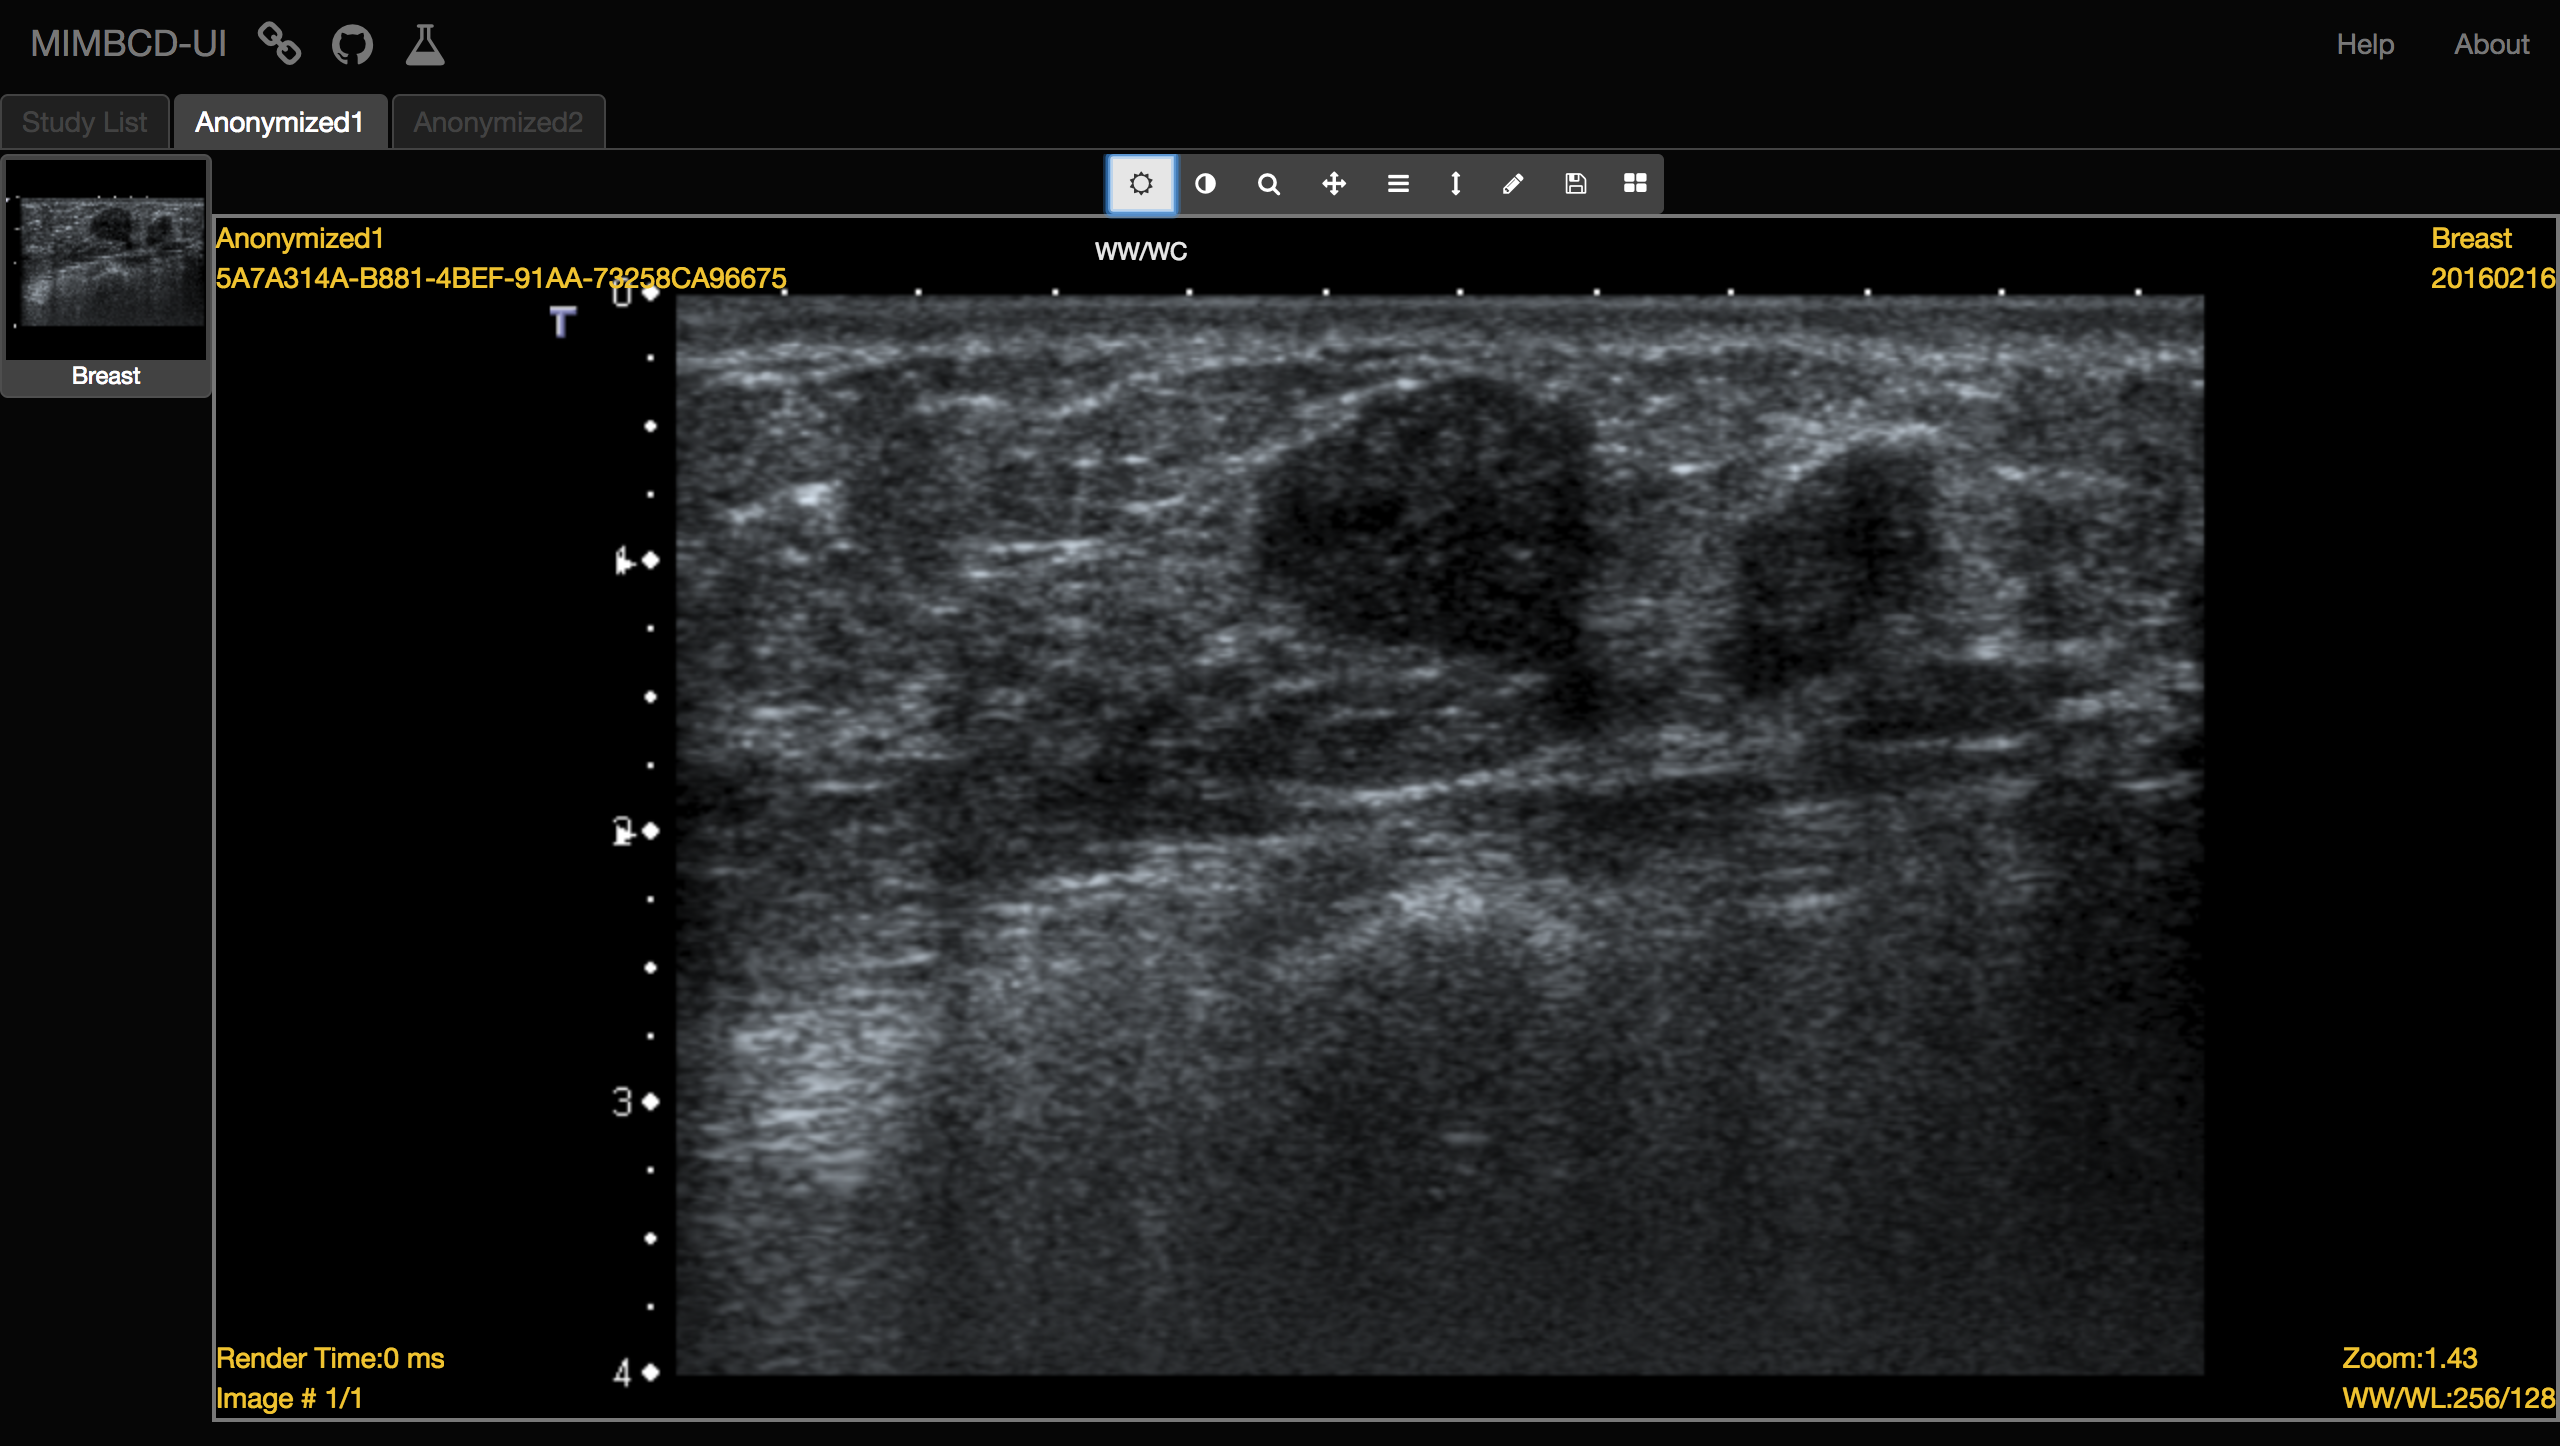
\includegraphics[width=0.75\textwidth]{graphics/anon1_ww_off.png}
\end{center}

\hfill

\clearpage

\item Drag down and up on the image viewer with the LEFT mouse button;

\hfill

\begin{center}
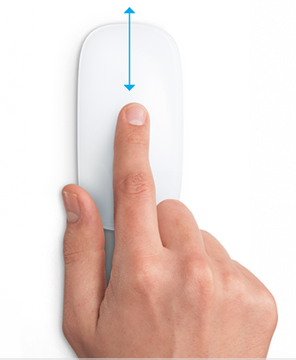
\includegraphics[width=0.50\textwidth]{graphics/mouse-up-down.png}
\end{center}

\hfill

\item Configure the pretended \textbf{WW/WC} level;

\hfill

\begin{center}
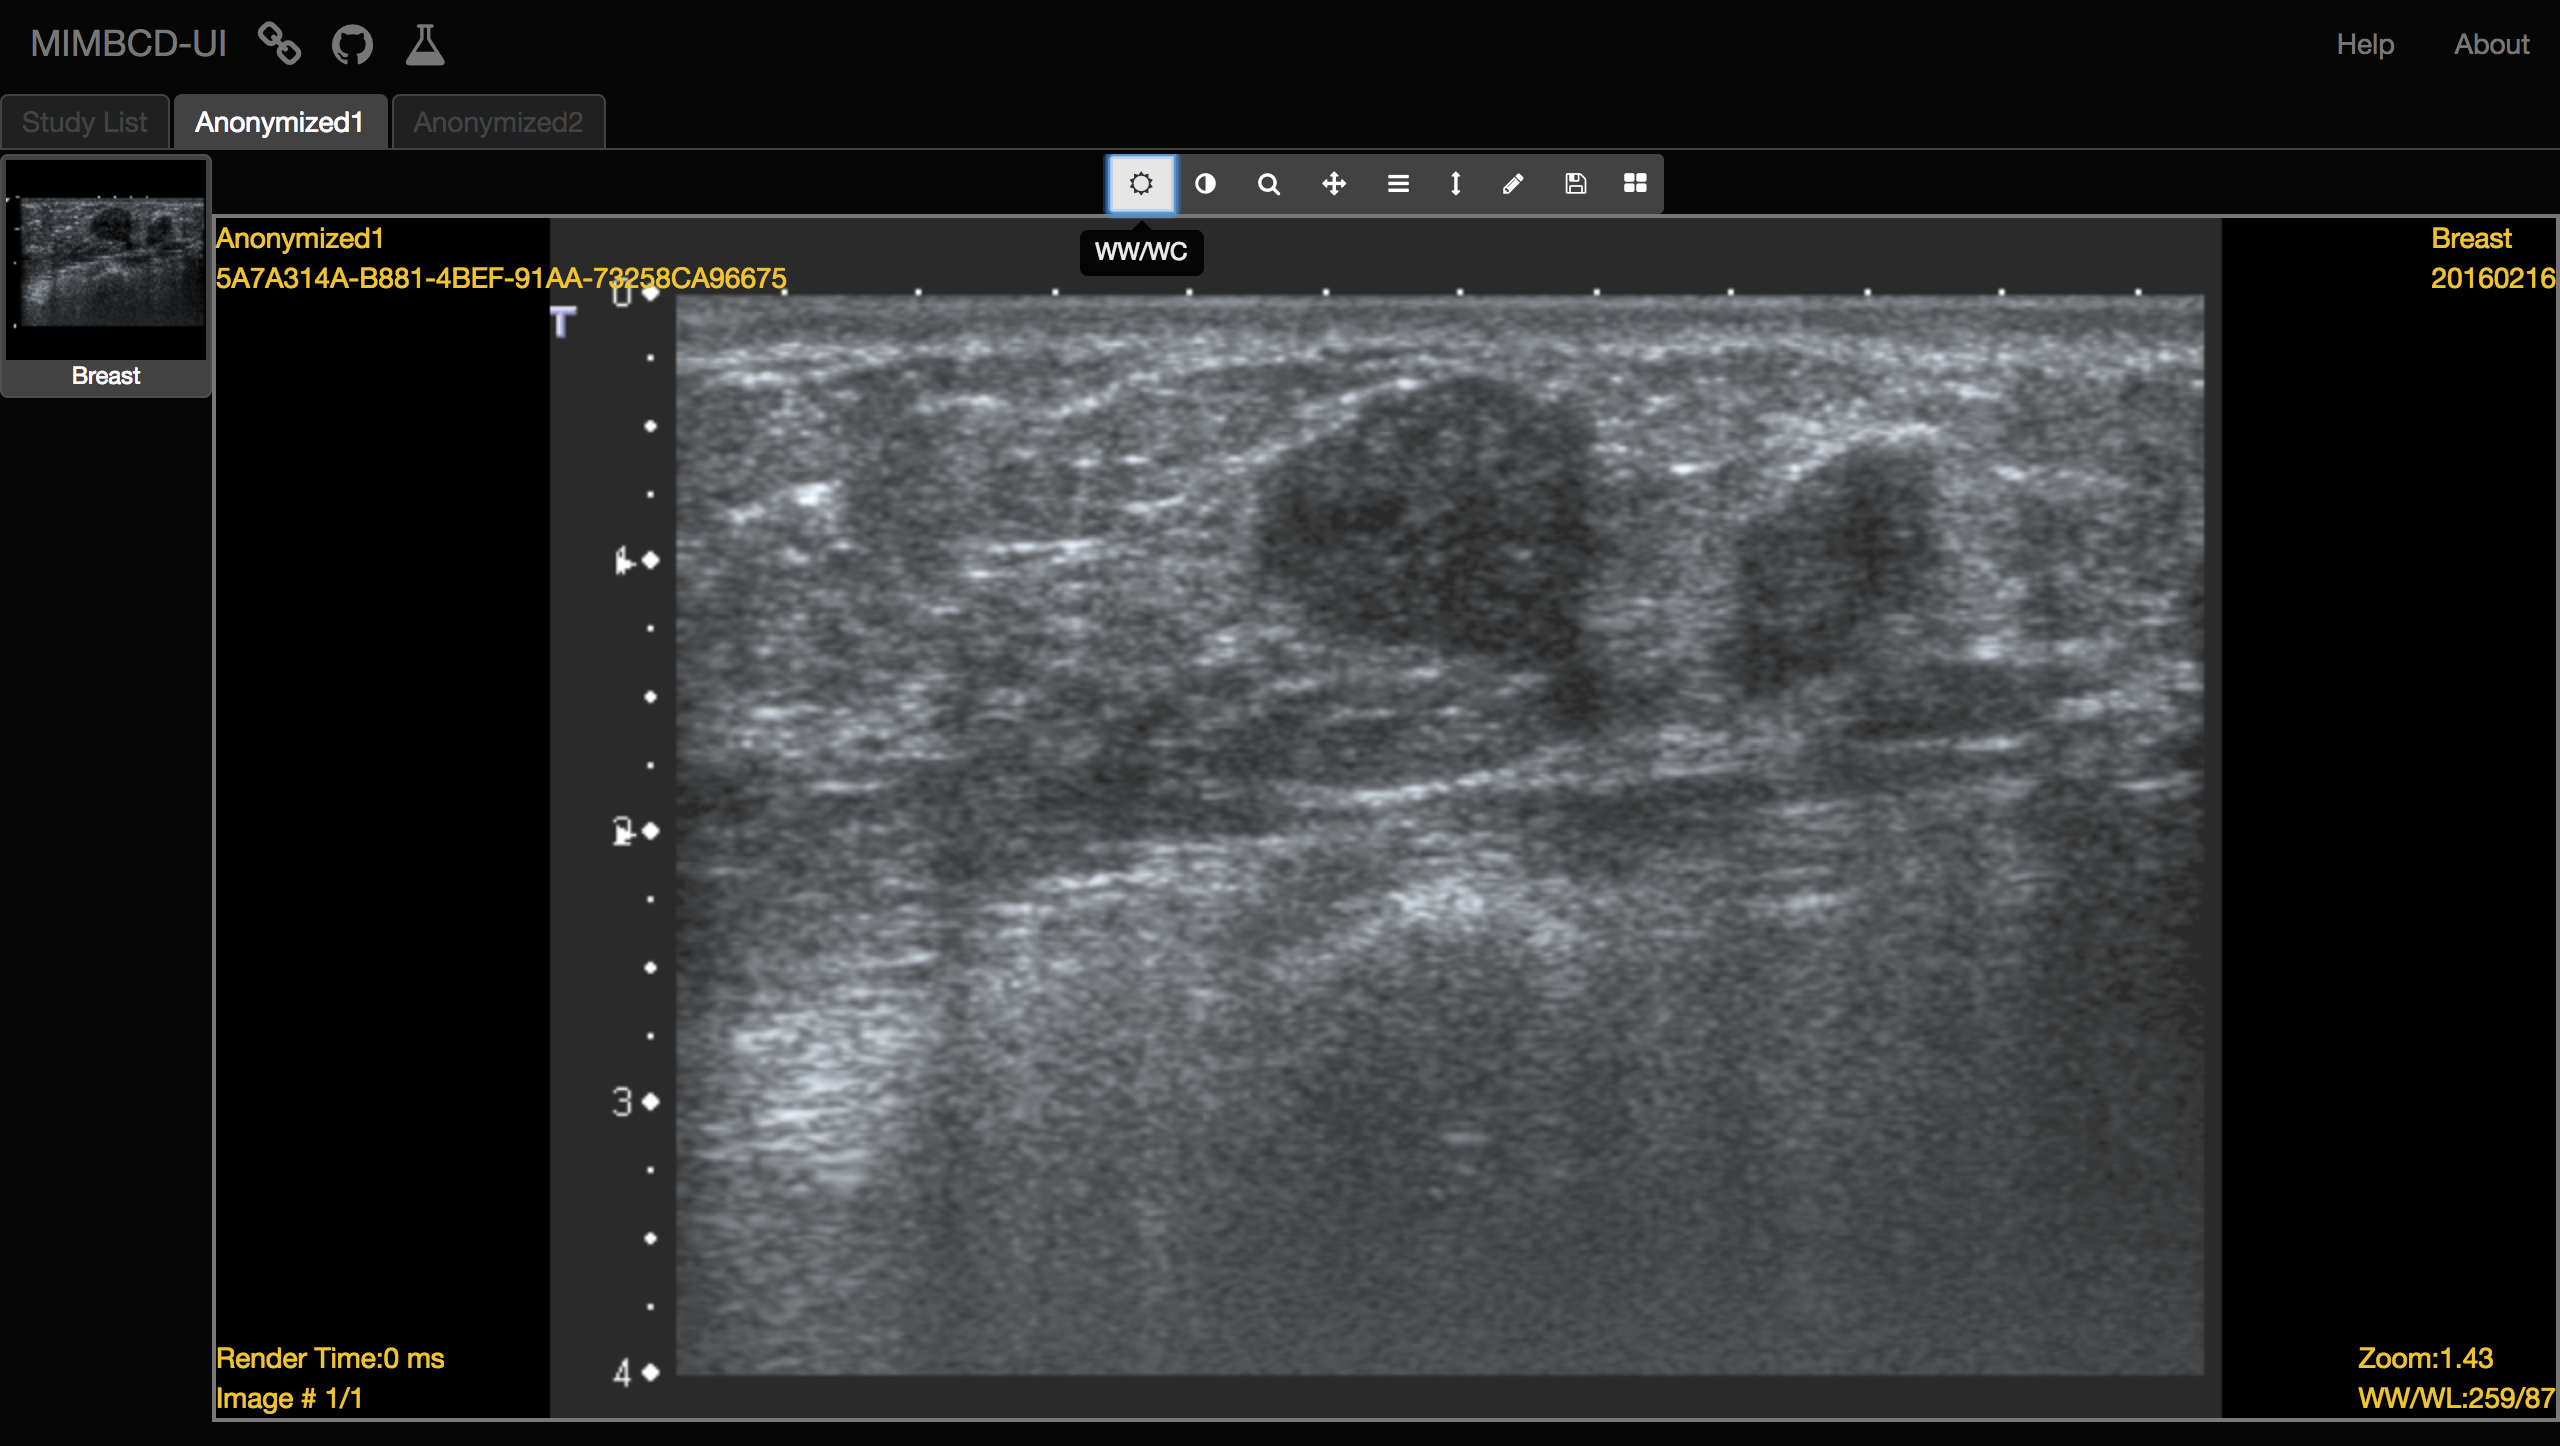
\includegraphics[width=0.75\textwidth]{graphics/anon1_ww_on.png}
\end{center}

\hfill

\end{enumerate}

% r.12 Invert
\chapter{Invert}

To flip the image in the active image viewer, click button and select \textbf{Invert} tool.

\hfill

\begin{center}
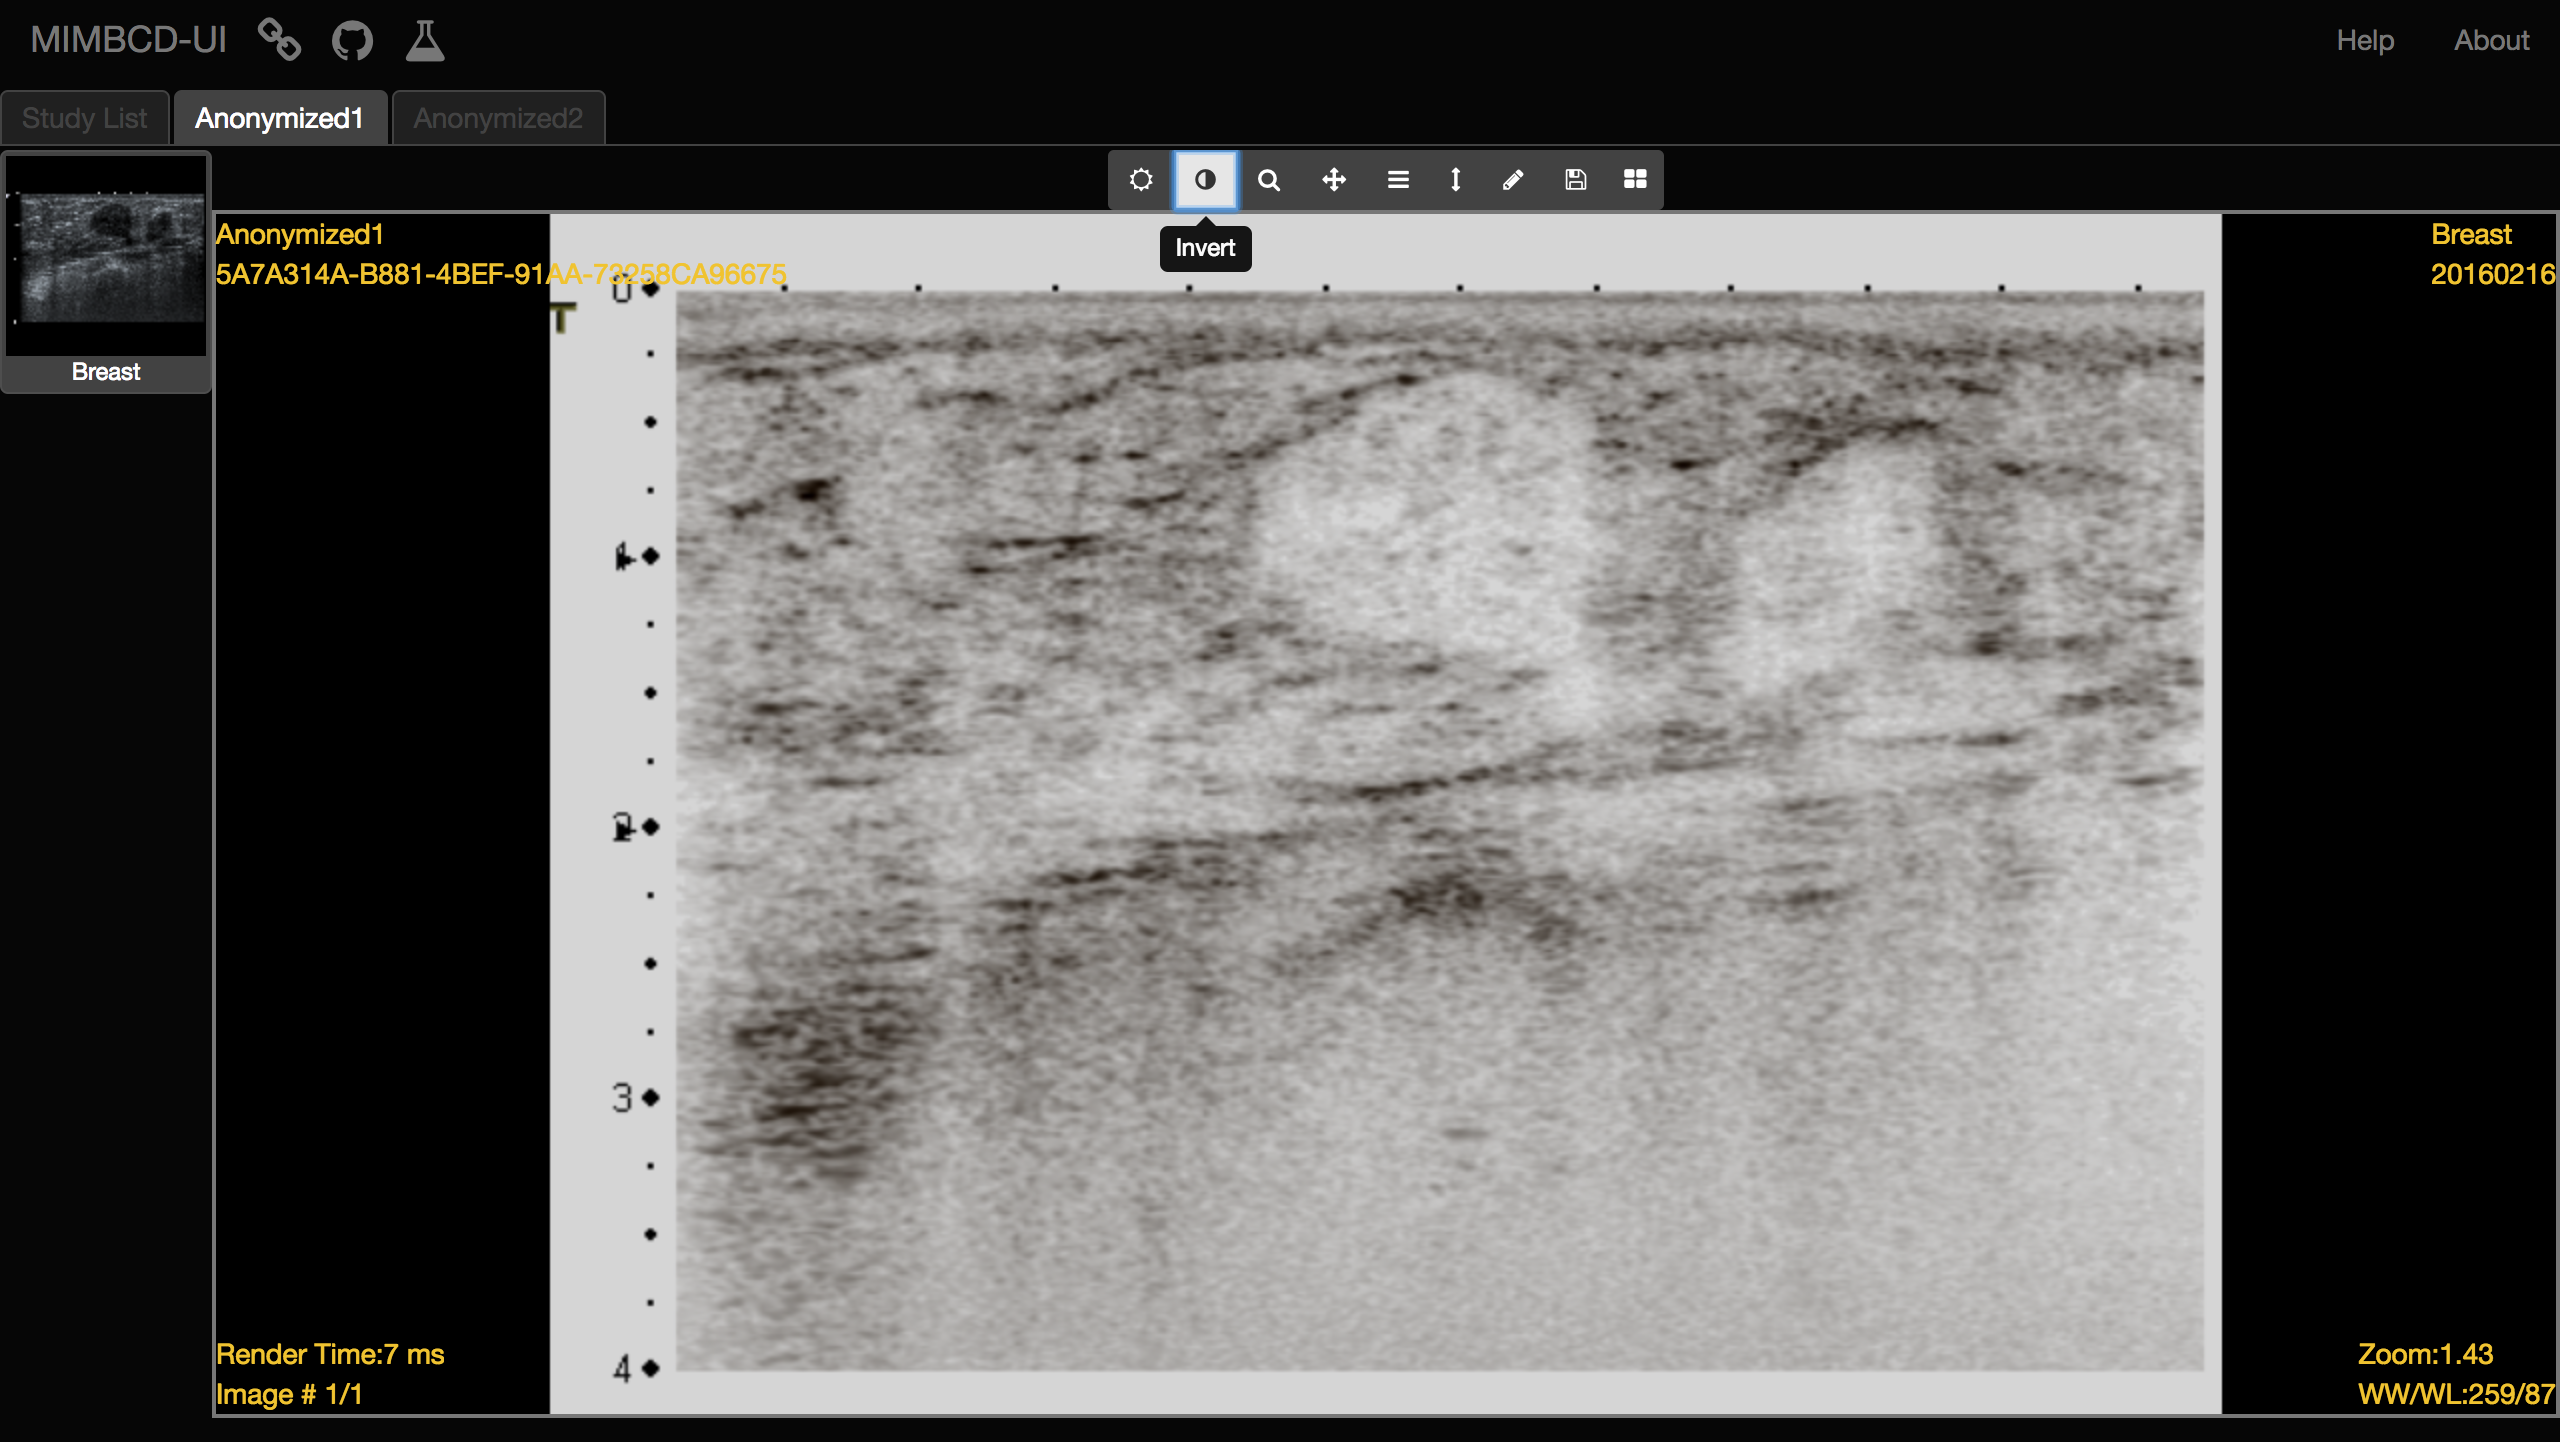
\includegraphics[width=\textwidth]{graphics/anon1_invert.png}
\end{center}

\hfill

\chapter{Zoom}

Select Zoom Tool and down on the image with the LEFT mouse button.

\begin{enumerate}

\item Select the \textbf{Zoom} option;

\begin{center}
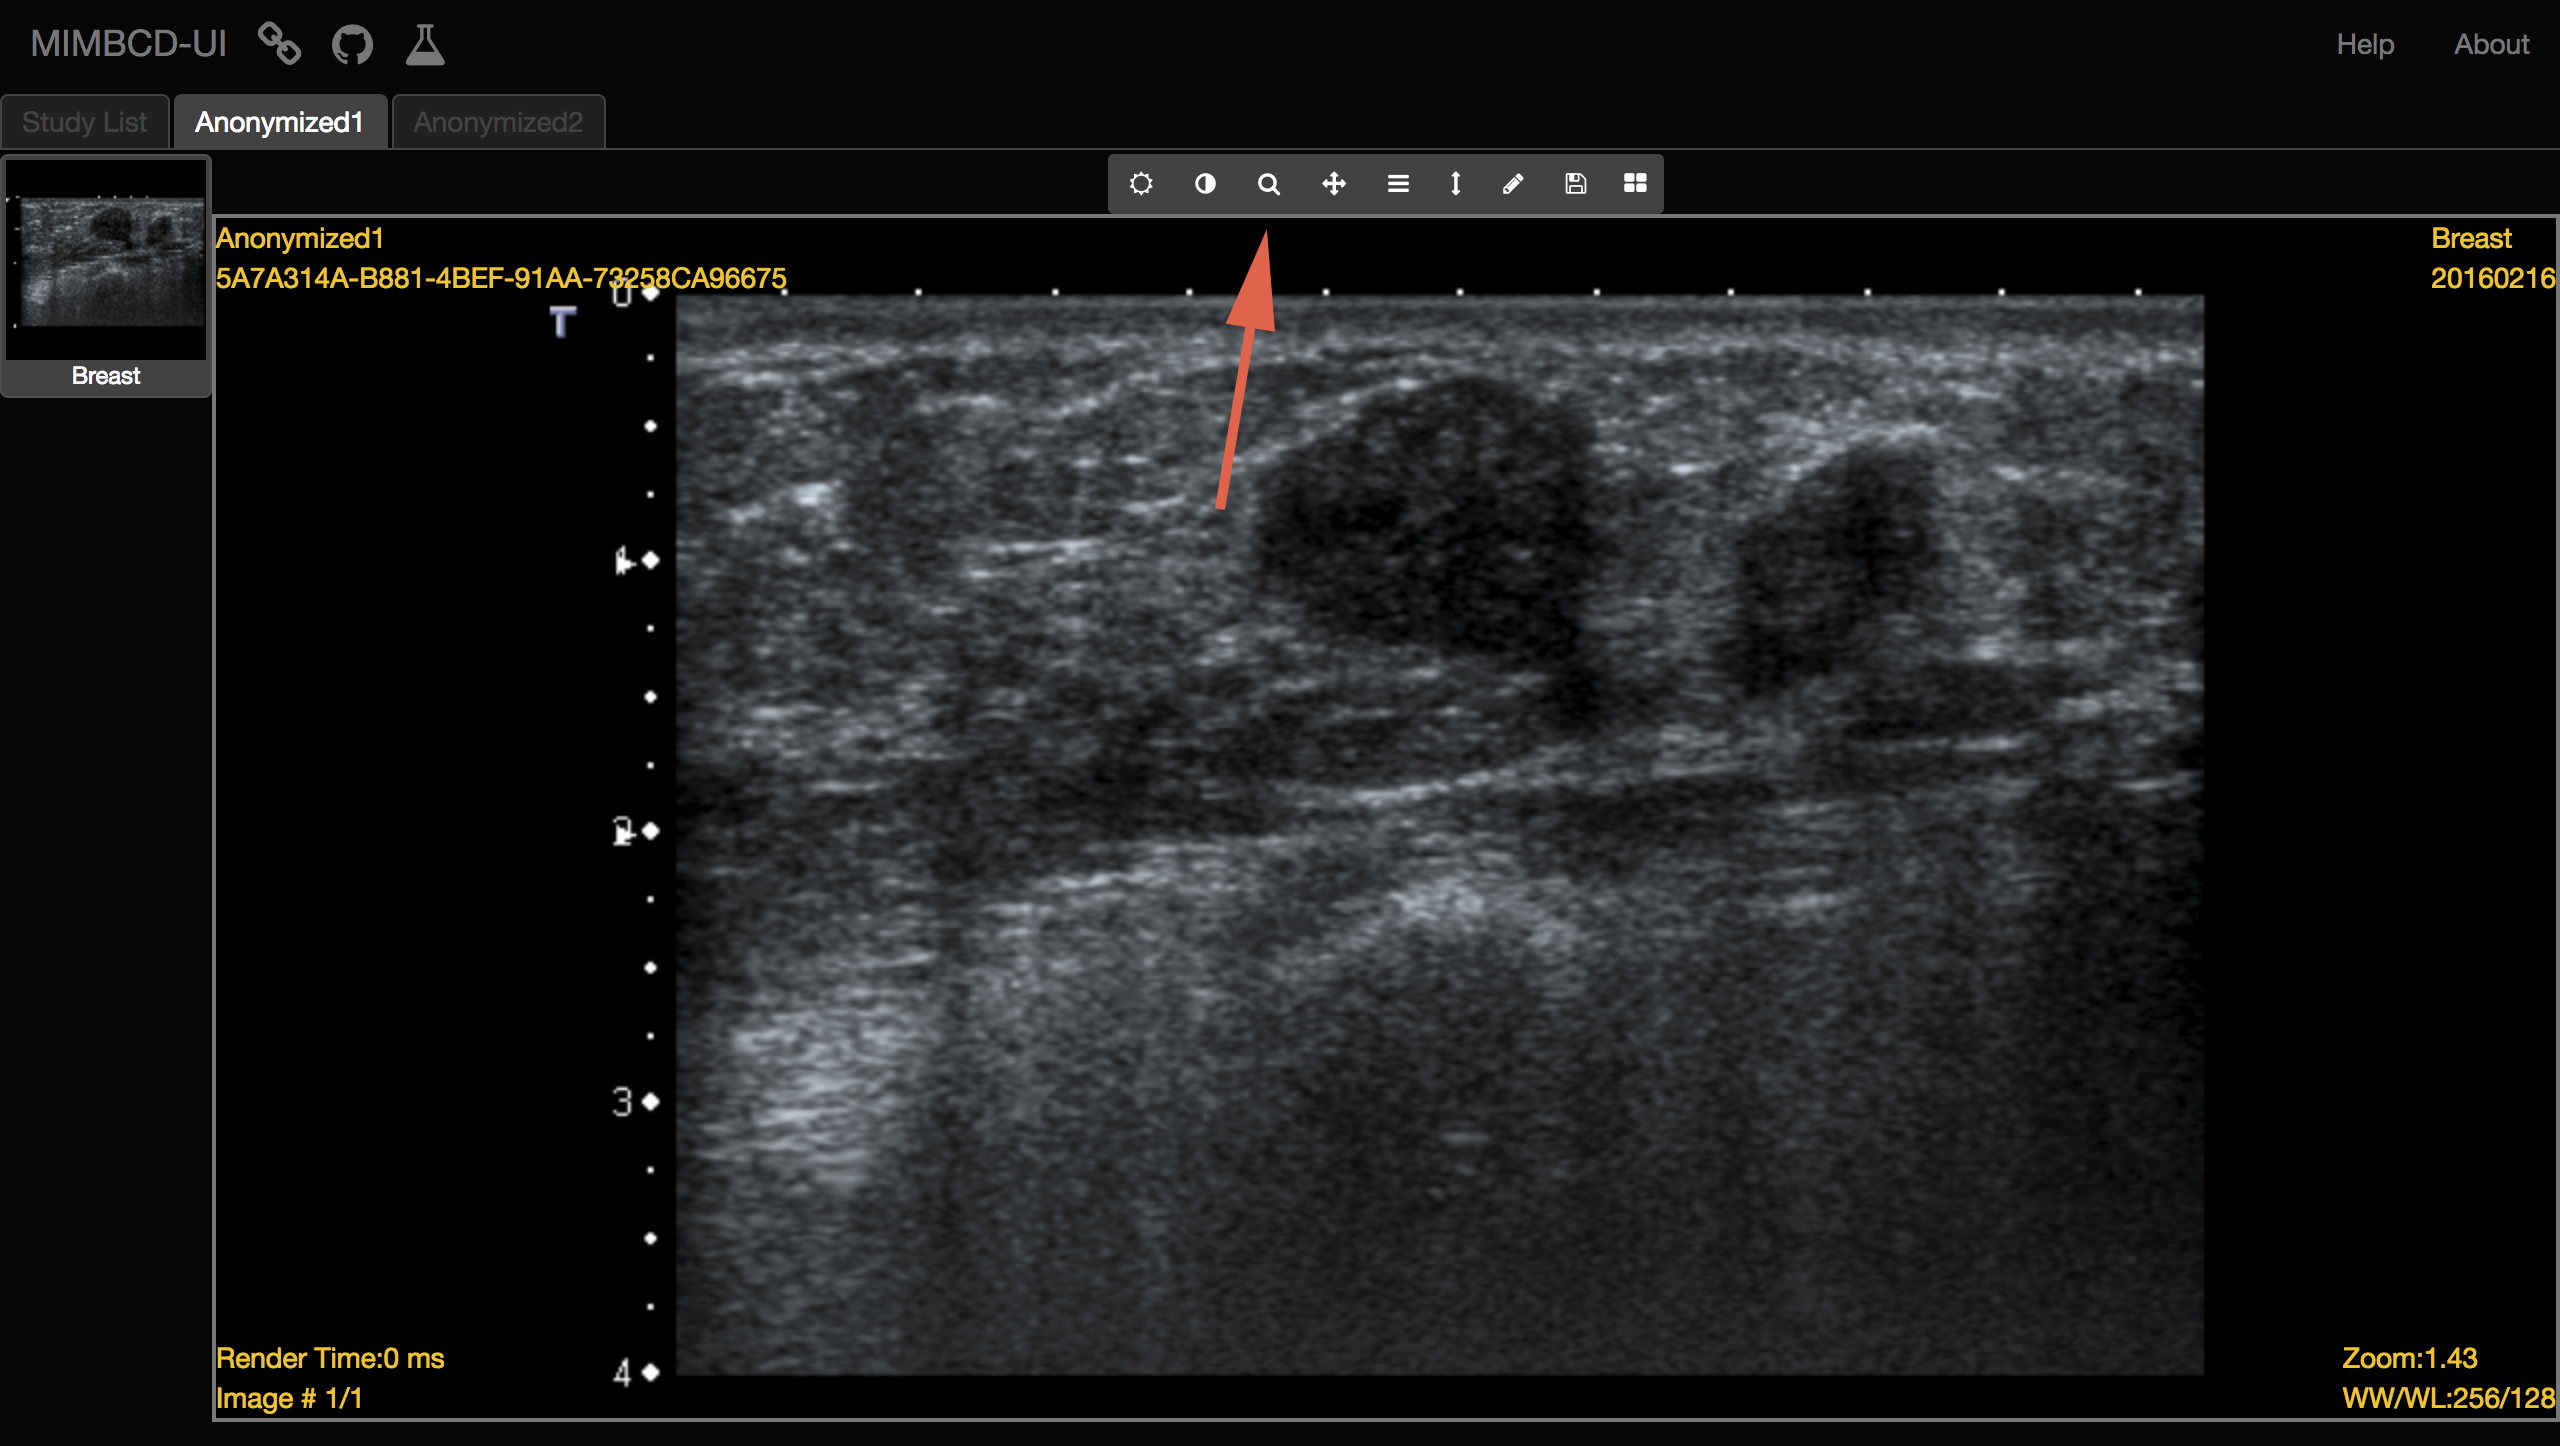
\includegraphics[width=0.75\textwidth]{graphics/anon1_zoom_out.png}
\end{center}

\item Drag down and up on the image viewer with the LEFT mouse button;

\begin{center}
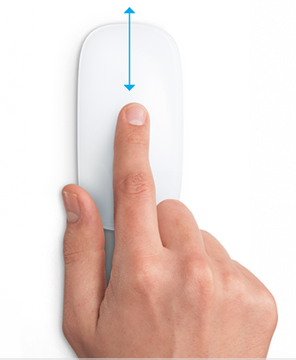
\includegraphics[width=0.50\textwidth]{graphics/mouse-up-down.png}
\end{center}

\item \textbf{Zoom} In and \textbf{Zoom} Out;

\begin{center}
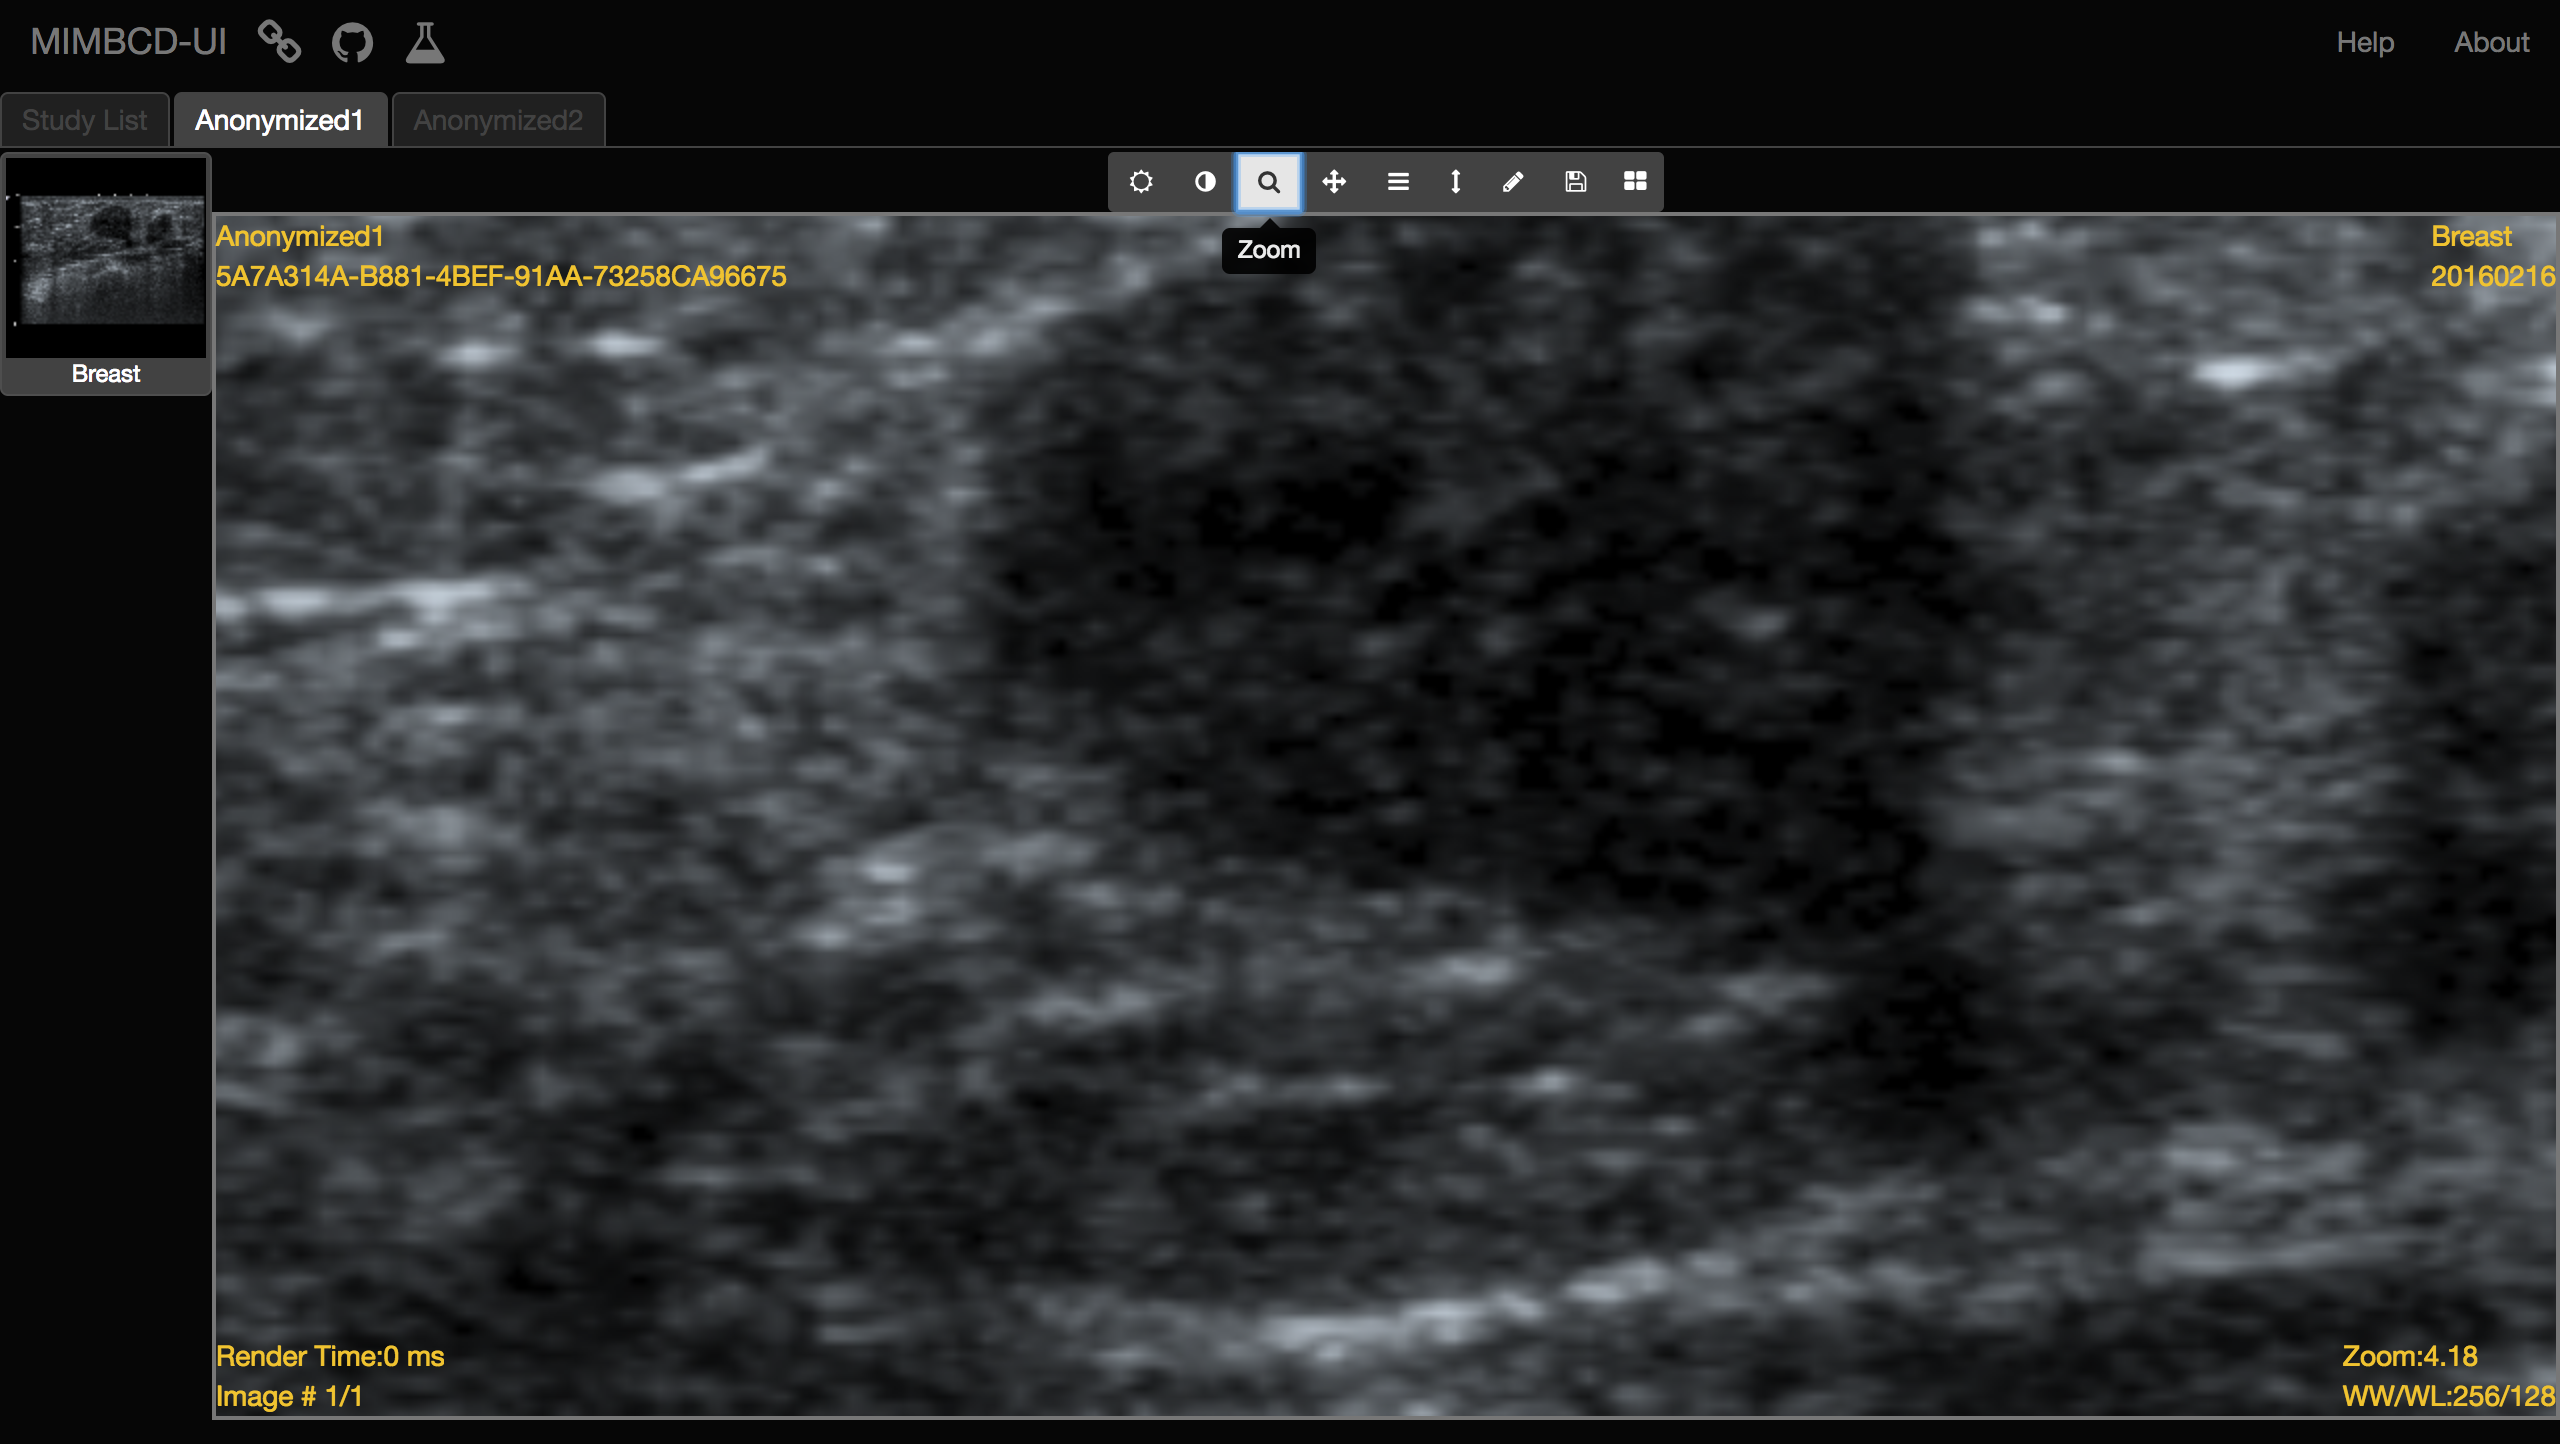
\includegraphics[width=0.75\textwidth]{graphics/anon1_zoom_in.png}
\end{center}

\end{enumerate}

% r.13 Pan
\chapter{Pan}

\begin{enumerate}

\item Select the \textbf{WW/WC} option;

\begin{center}
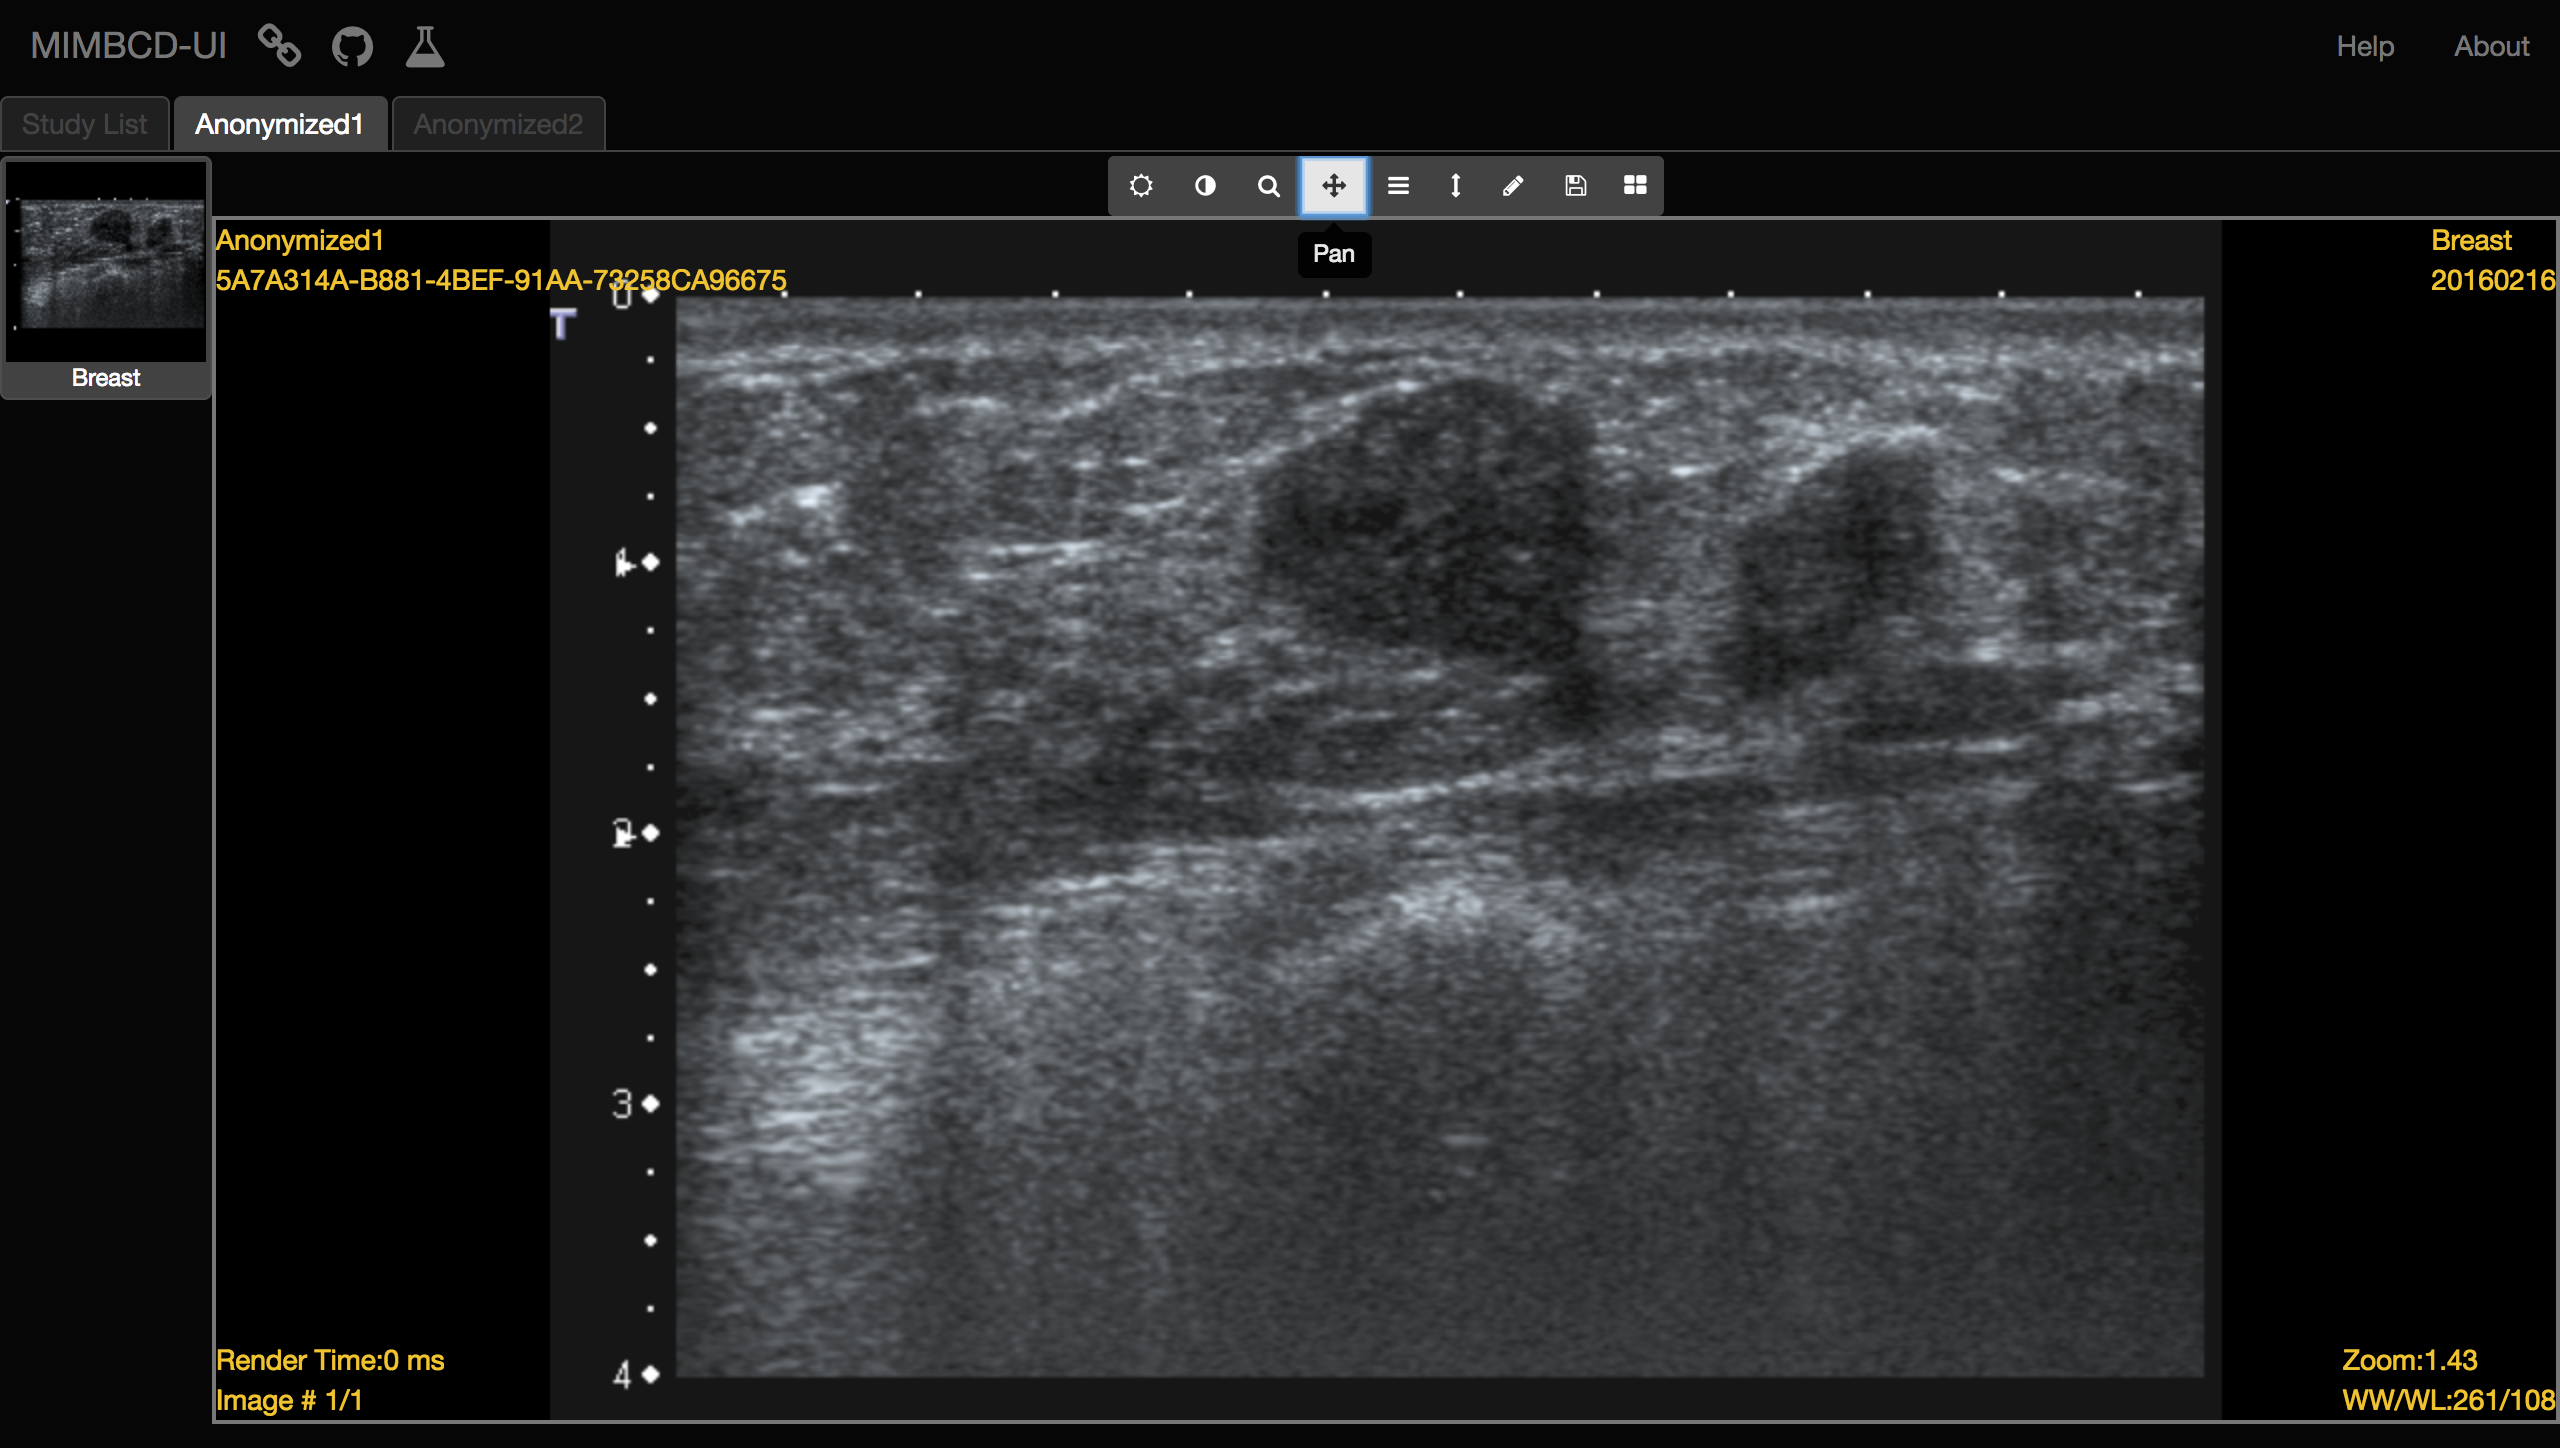
\includegraphics[width=0.75\textwidth]{graphics/anon1_pan_off.png}
\end{center}

\item Drag the image down and up, left and right on the image viewer with the LEFT mouse button;

\begin{center}
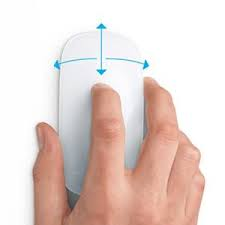
\includegraphics[width=0.50\textwidth]{graphics/mouse-all.png}
\end{center}

\item Positioning of the image;

\begin{center}
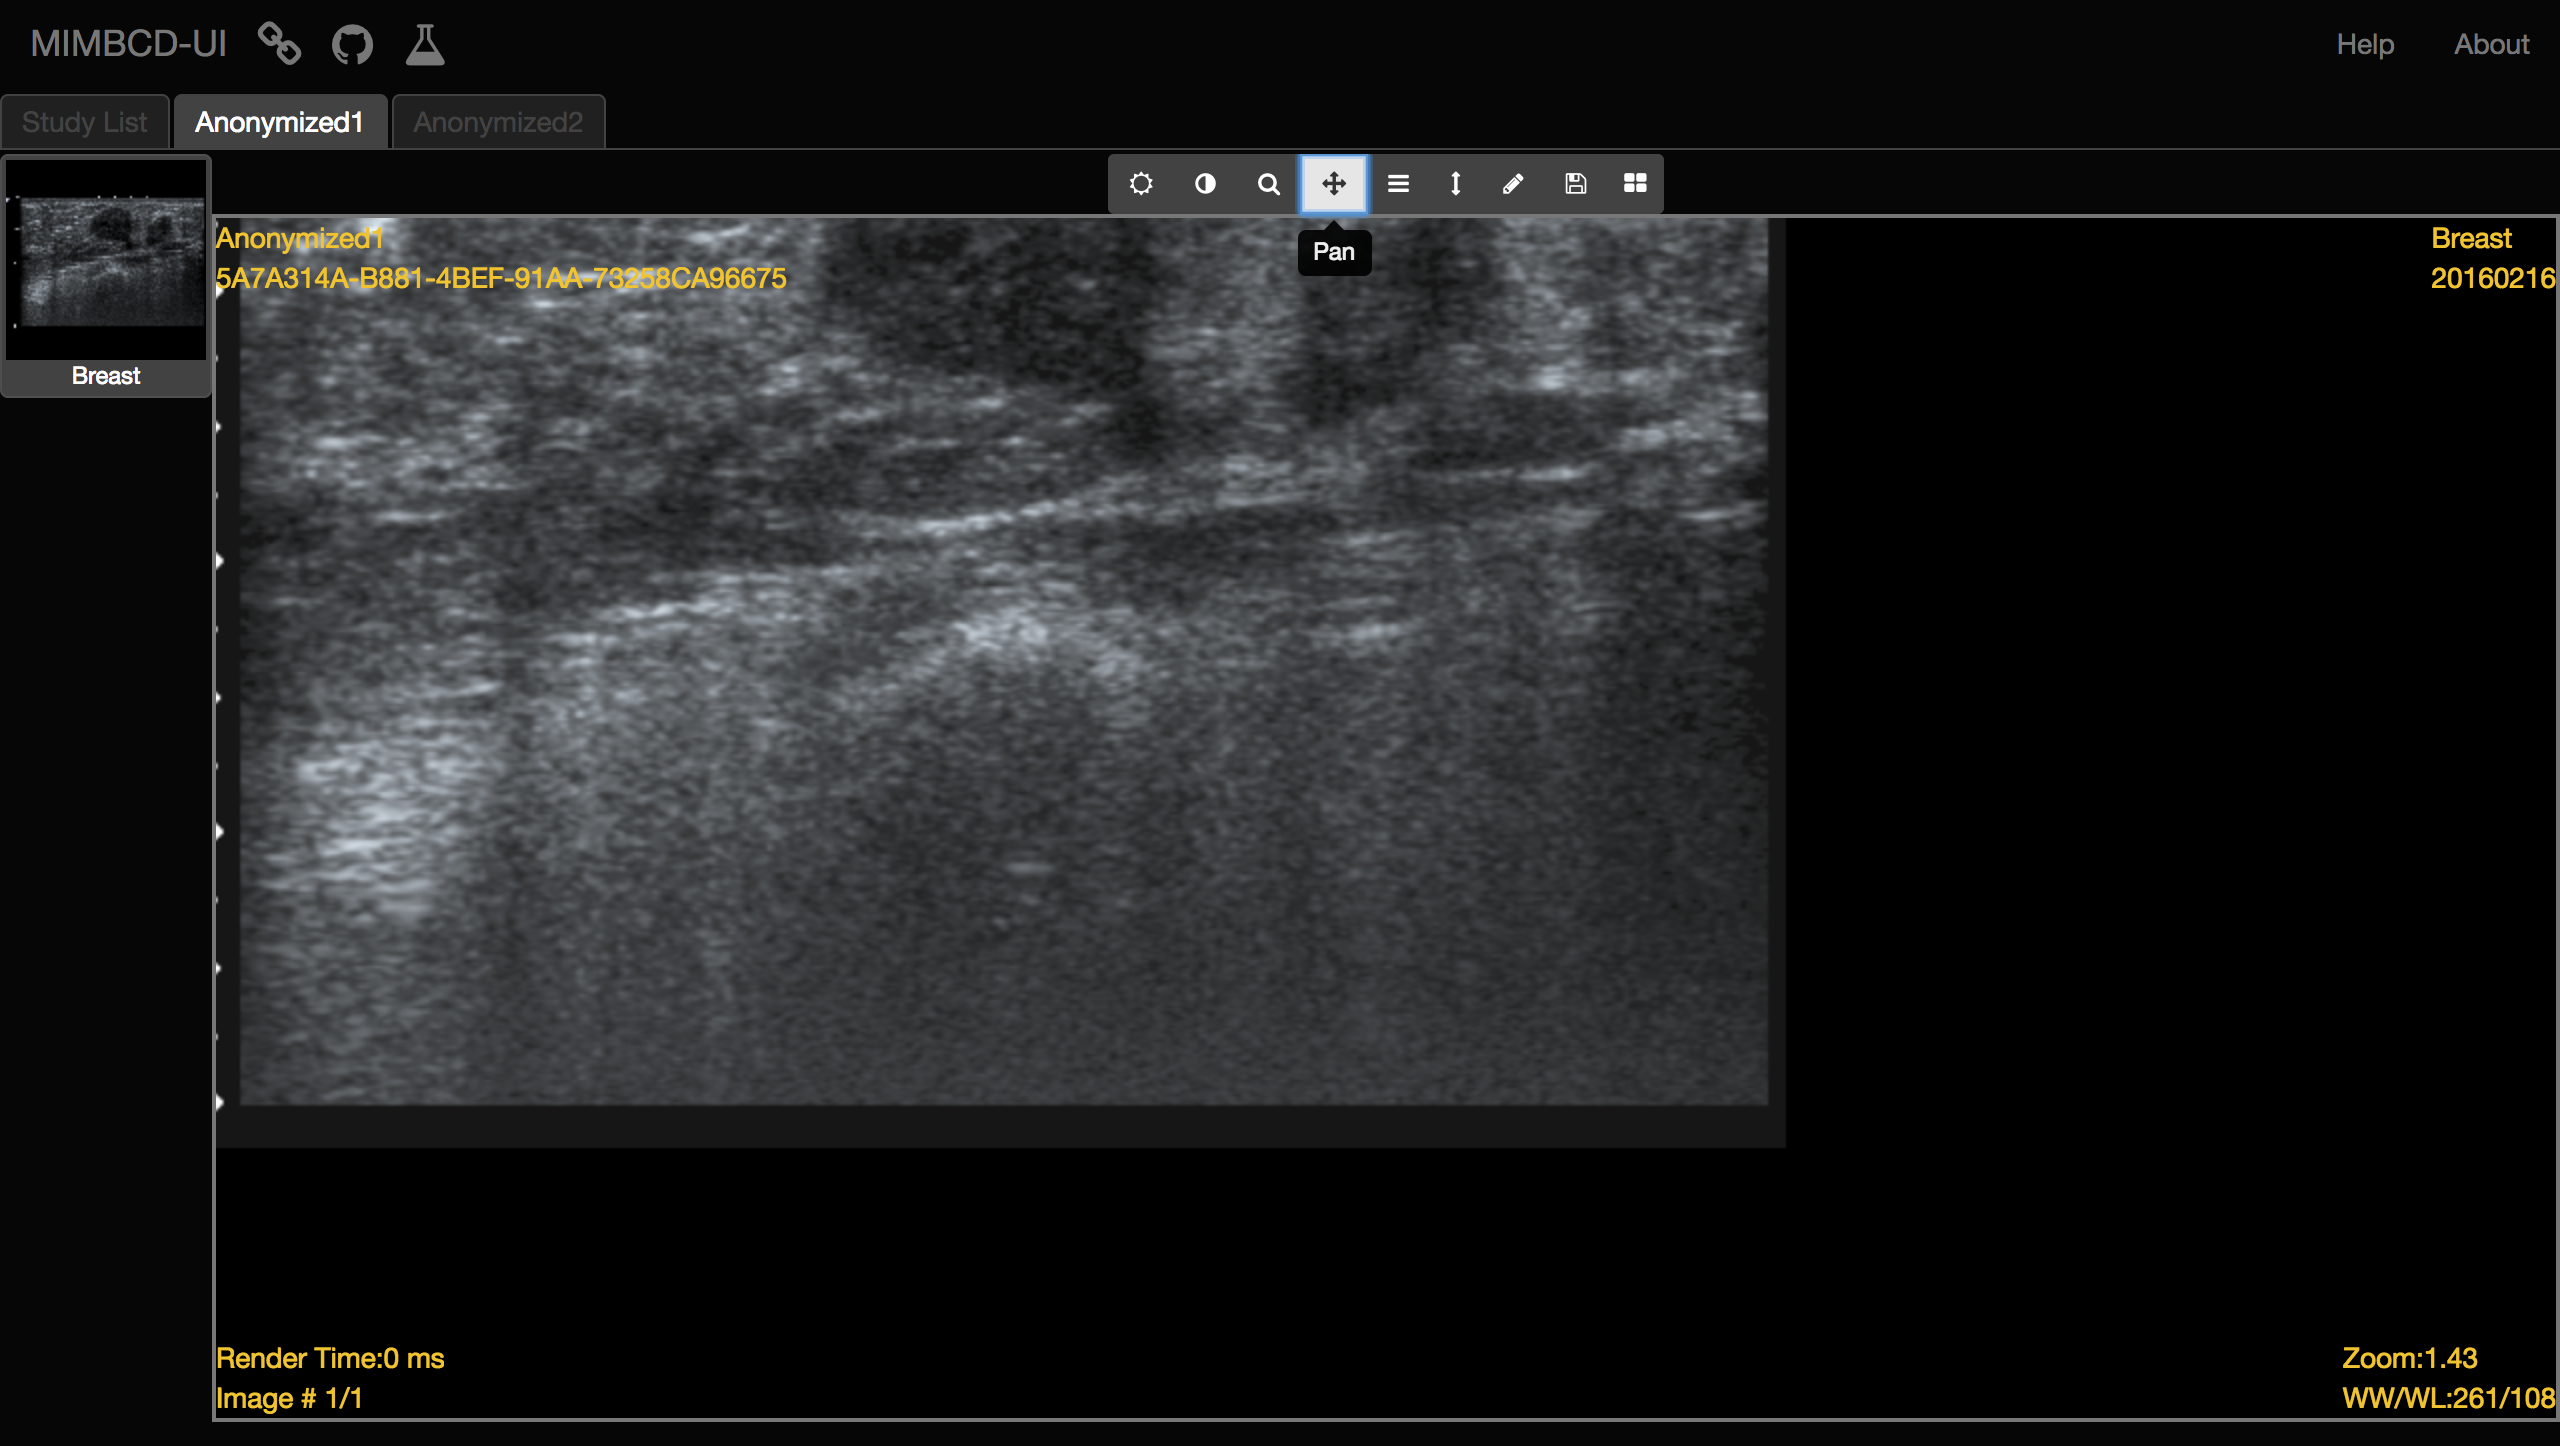
\includegraphics[width=0.75\textwidth]{graphics/anon1_pan_on.png}
\end{center}

\end{enumerate}

% r.14 Stack Scroll
\chapter{Stack Scroll}

An image \textbf{Stack Scroll} is a feature to scroll over a collection of one or more images that are closely related. The best example of this is a CT or MRI series. A stack can include all images in a series or a subset of them. A stack can even include images from different series in different studies. To use this feature over your images just follow the next instructions.

\begin{enumerate}

\item Click More button and select Stack Scroll Tool;

\item Drag down and up on the image viewer with the left mouse button;

\hfill

\begin{center}
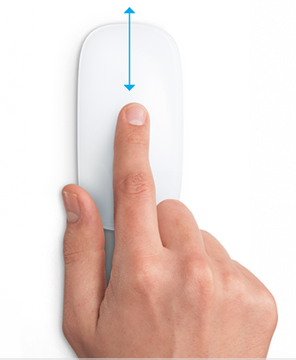
\includegraphics[width=0.50\textwidth]{graphics/mouse-up-down.png}
\end{center}

\hfill

\end{enumerate}

% r.15 Length
\chapter{Length}

To measure a lesion, click \textbf{Length} button at the Menu Bar of the workspace. The \textbf{Length} feature will be displayed at the right side of the workspace.

\begin{center}
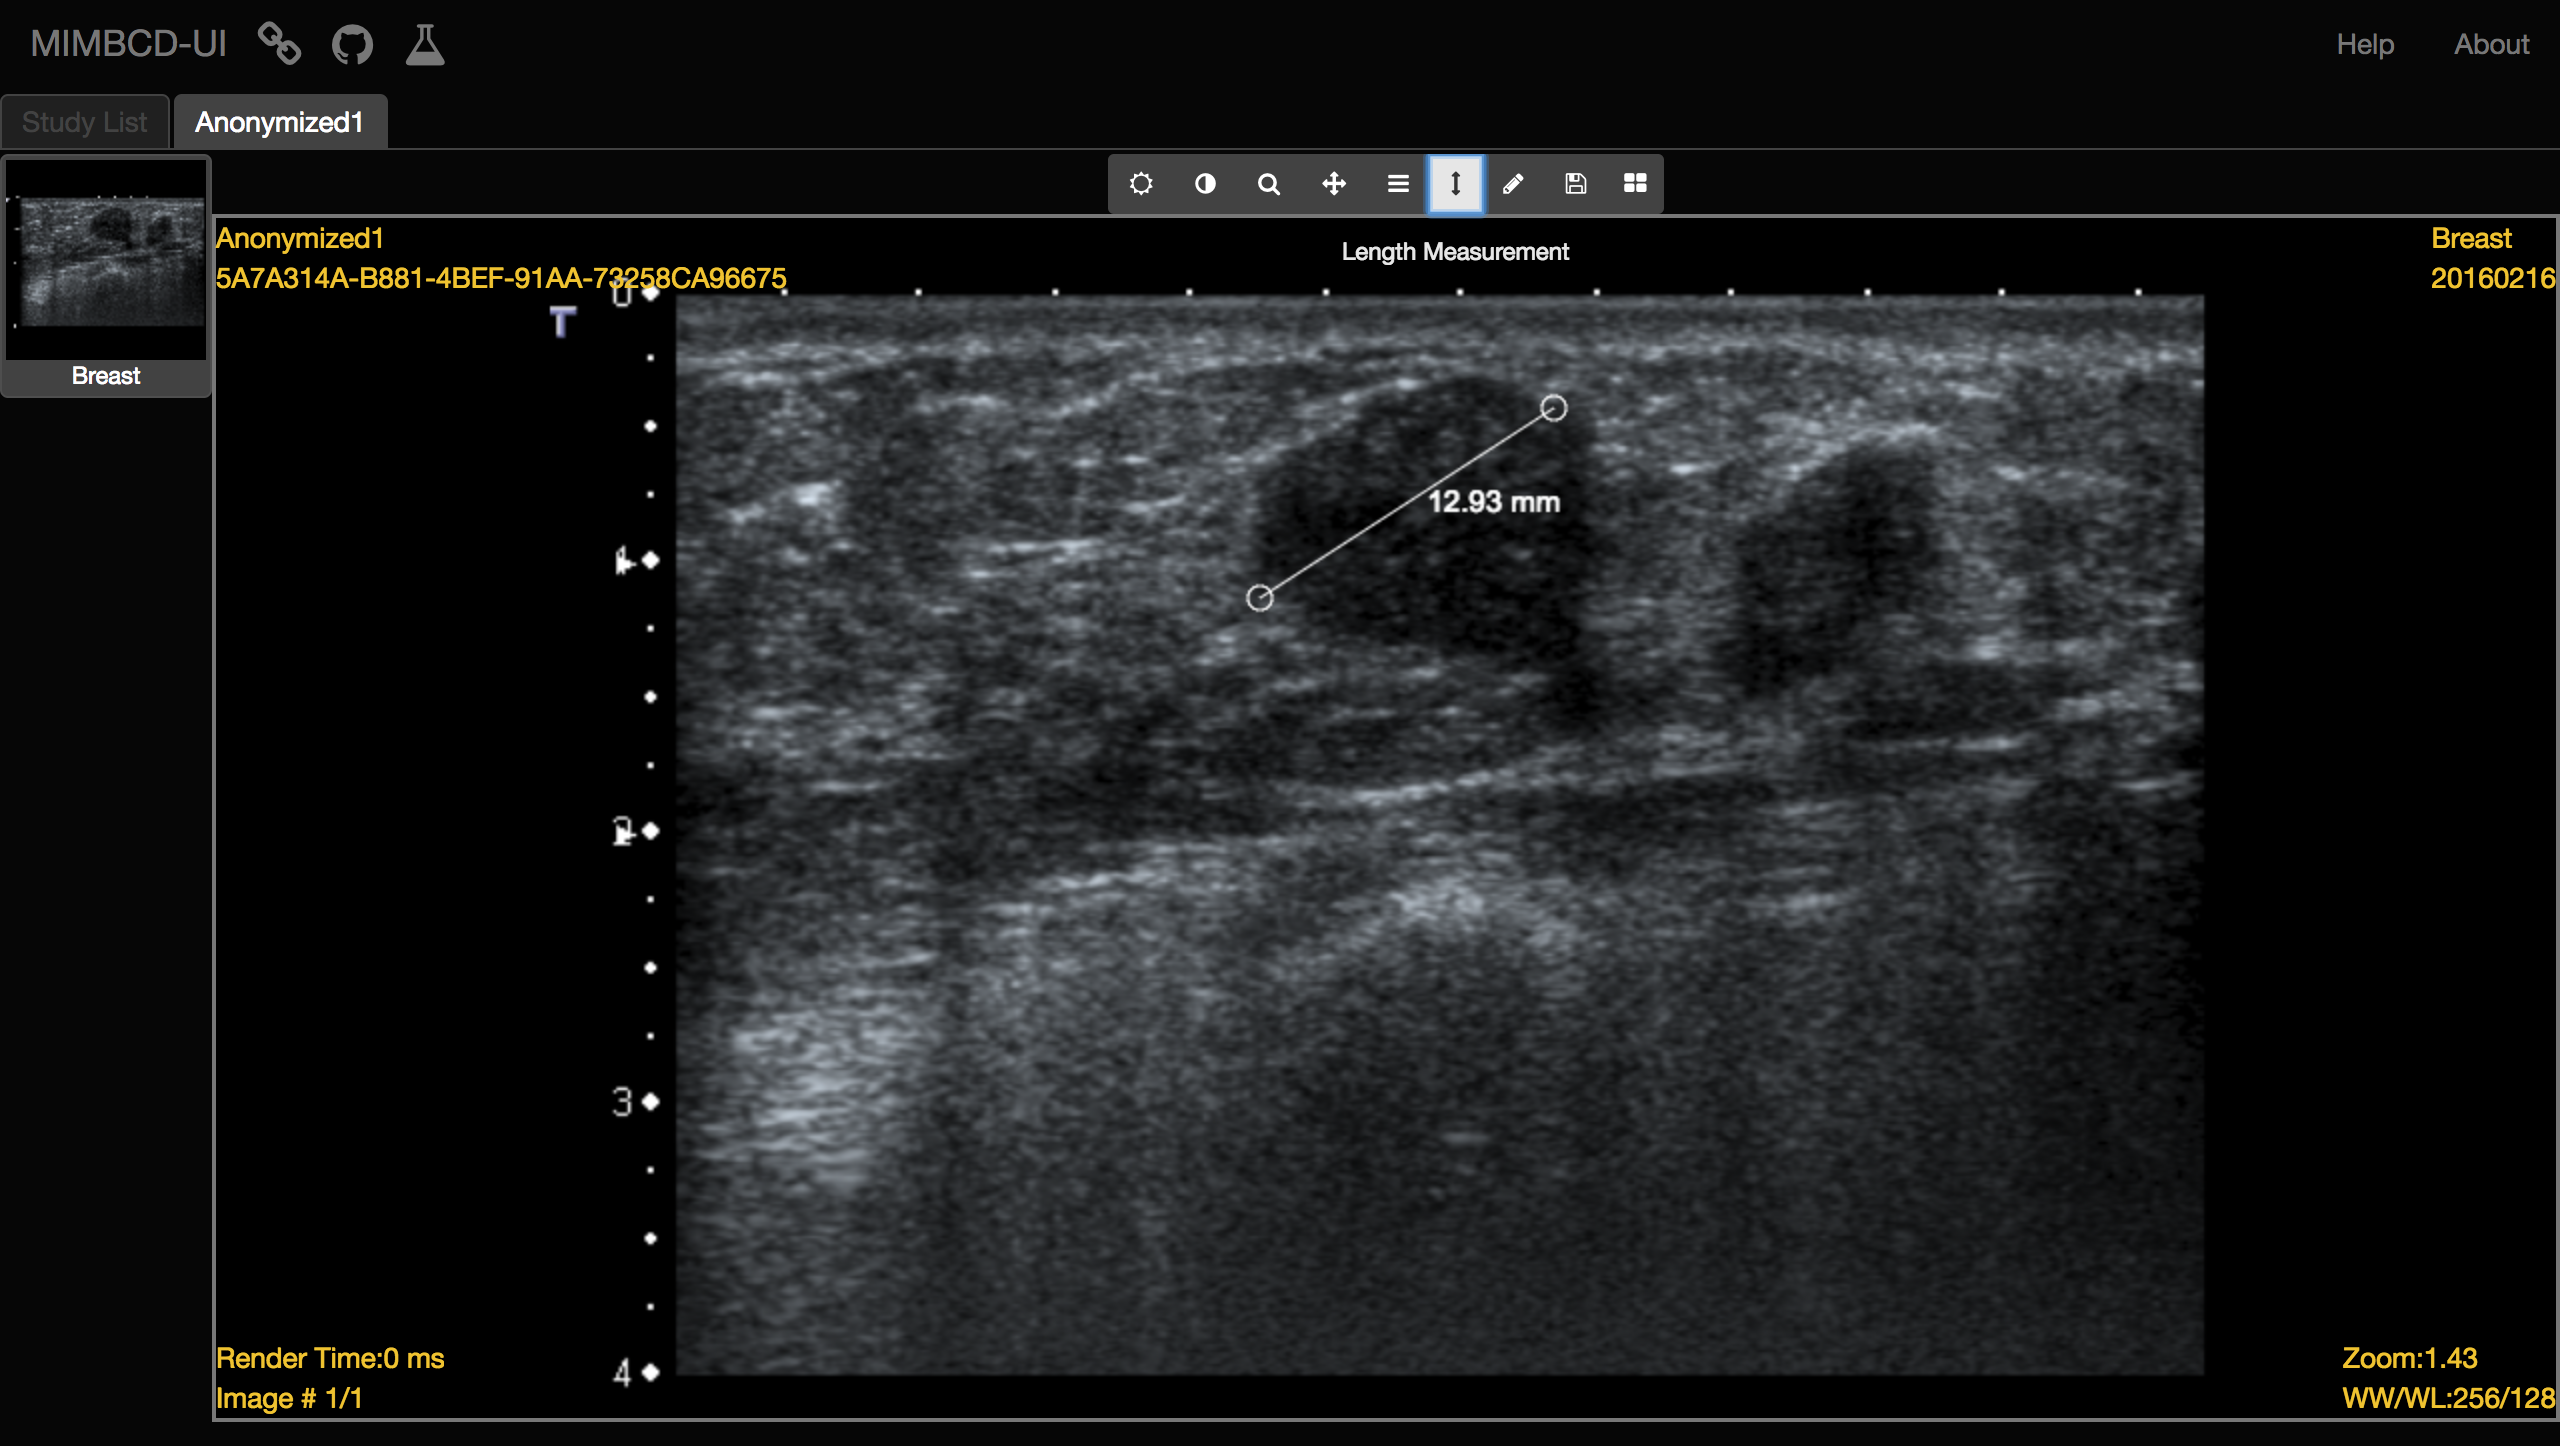
\includegraphics[width=\textwidth]{graphics/anon1_length.png}
\end{center}

% r.16 Windows
\chapter{Windows}

There are a number of default \textbf{Windows} settings in the \textbf{Windows} tab. To create a new setting, enter the desired column field.

\begin{center}
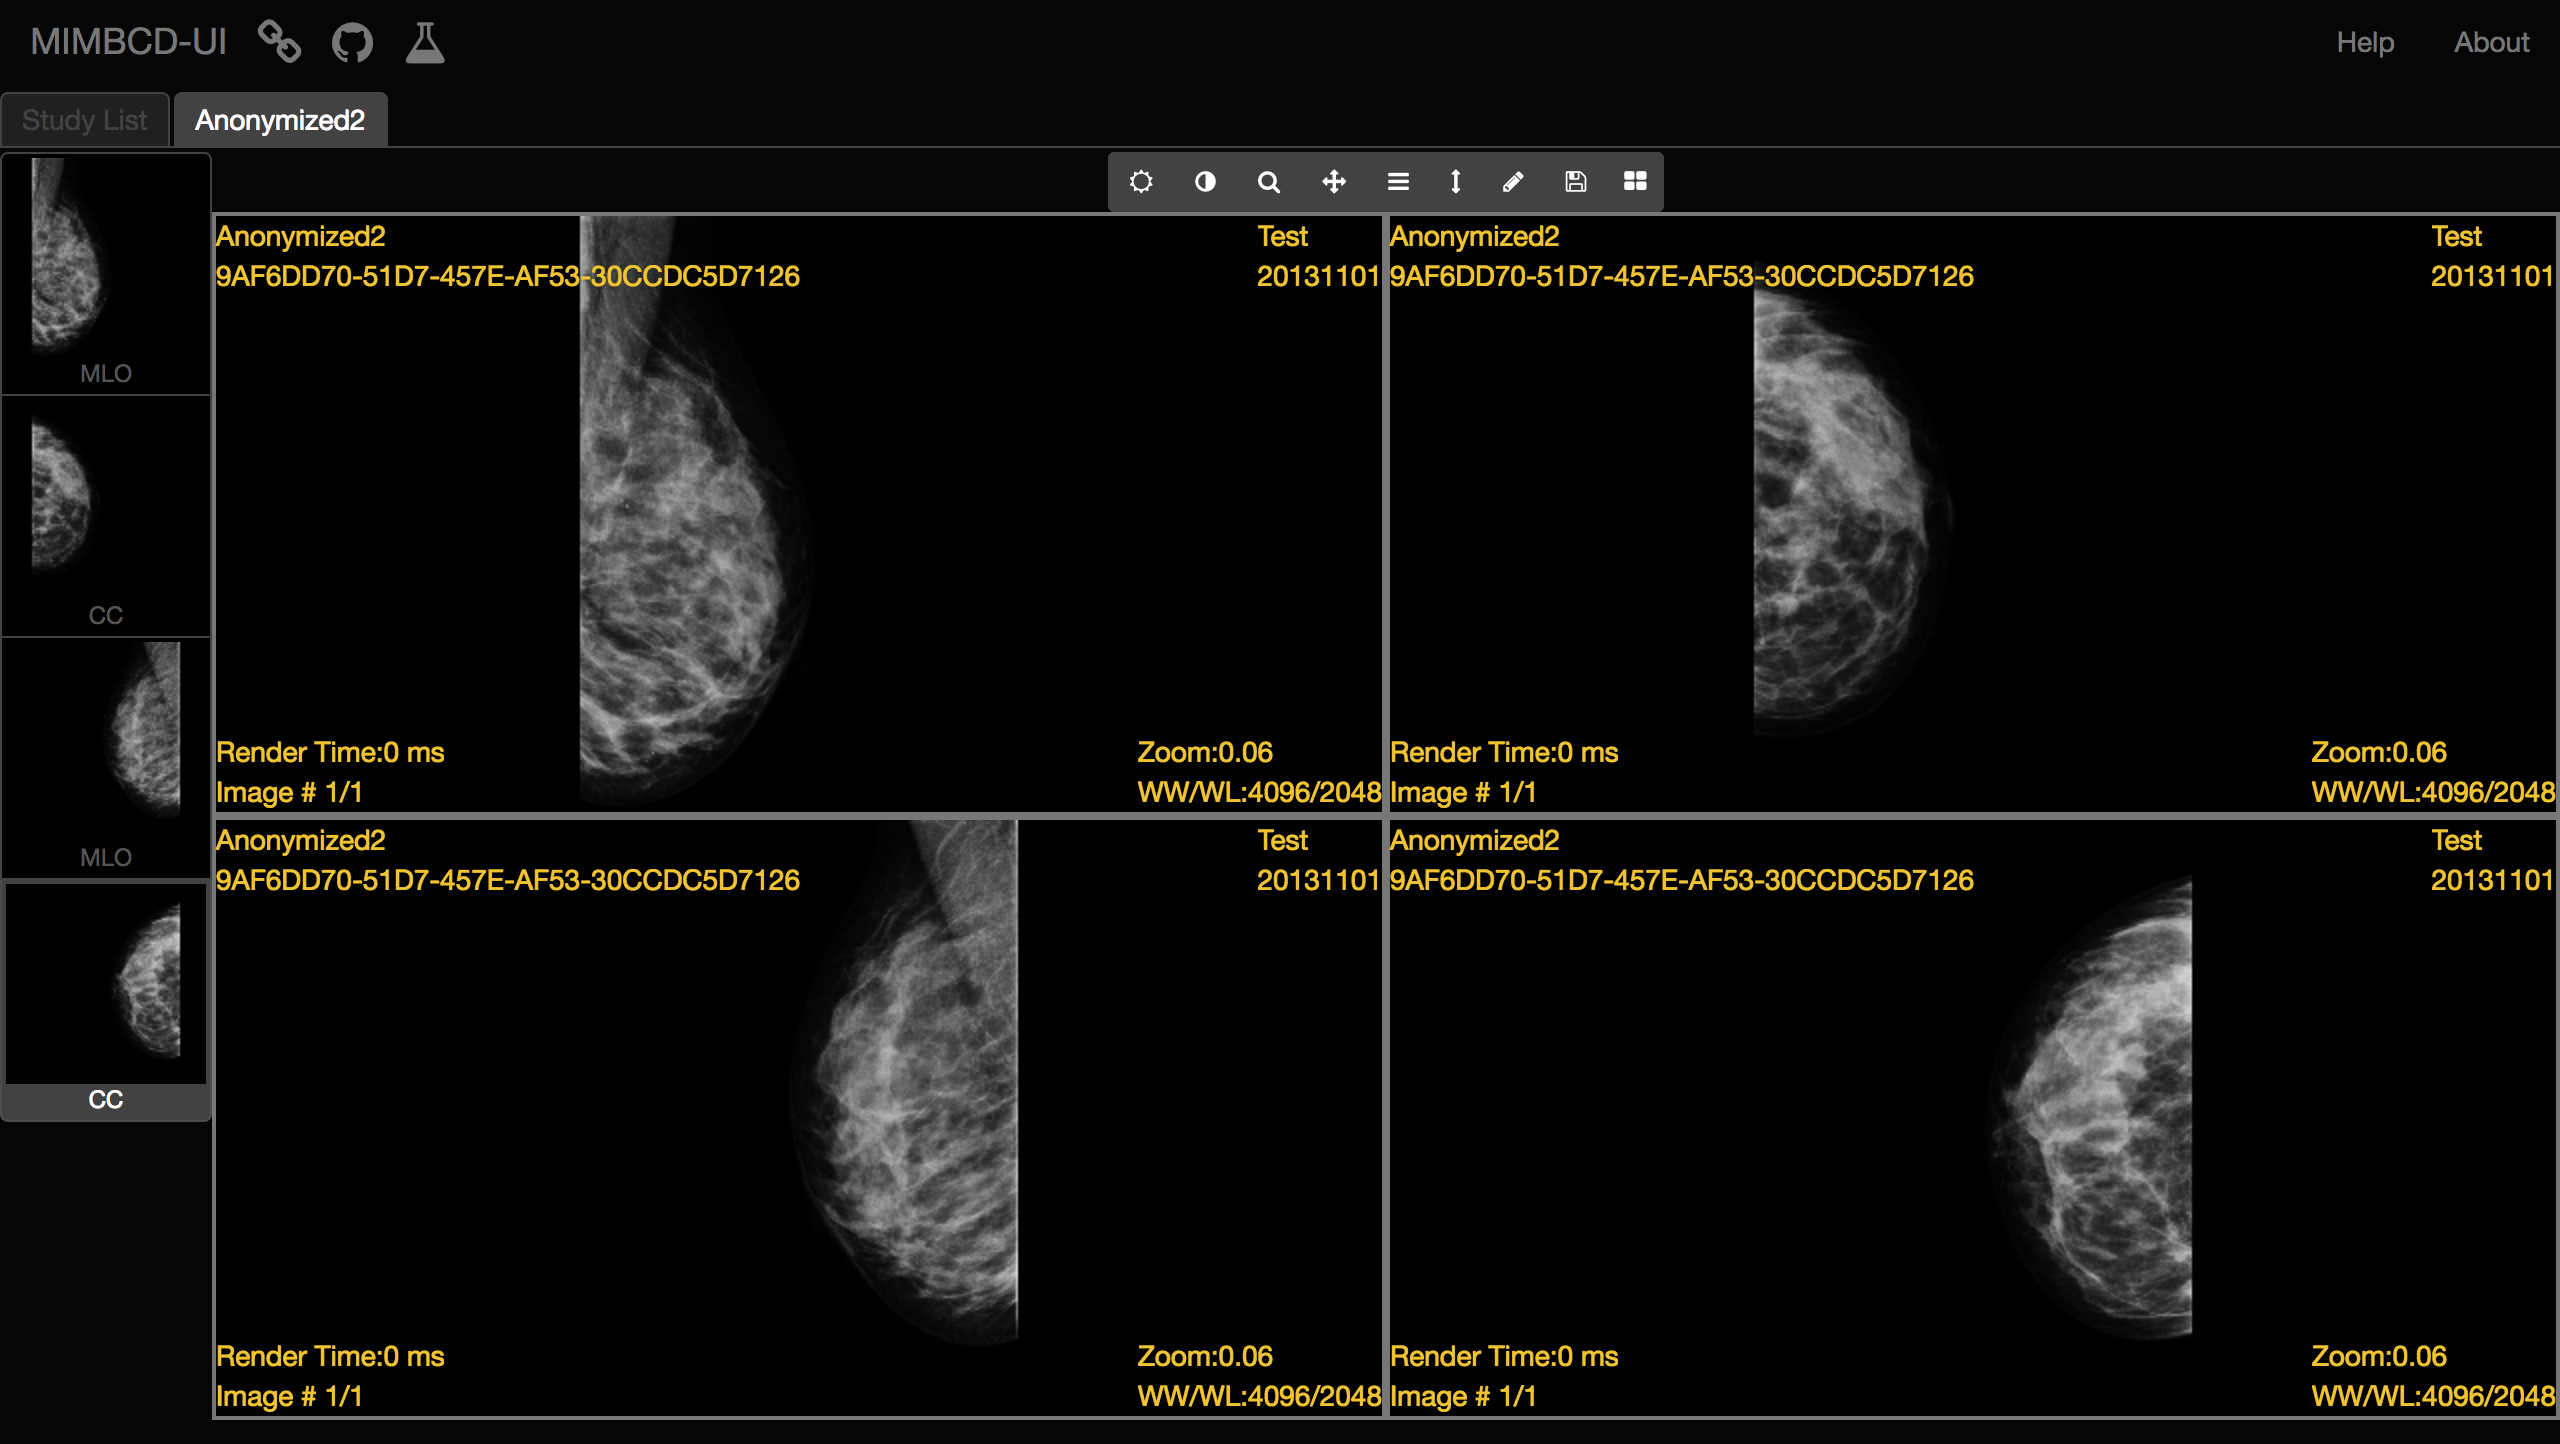
\includegraphics[width=\textwidth]{graphics/anon1_windows.png}
\end{center}

% r.17 Freehand
\chapter{Freehand}

To annotate a lesion, click \textbf{Freehand} and annotate the number of marks as you want:

\begin{enumerate}

\item Select the \textbf{Freehand} option and start annotating;

\begin{center}
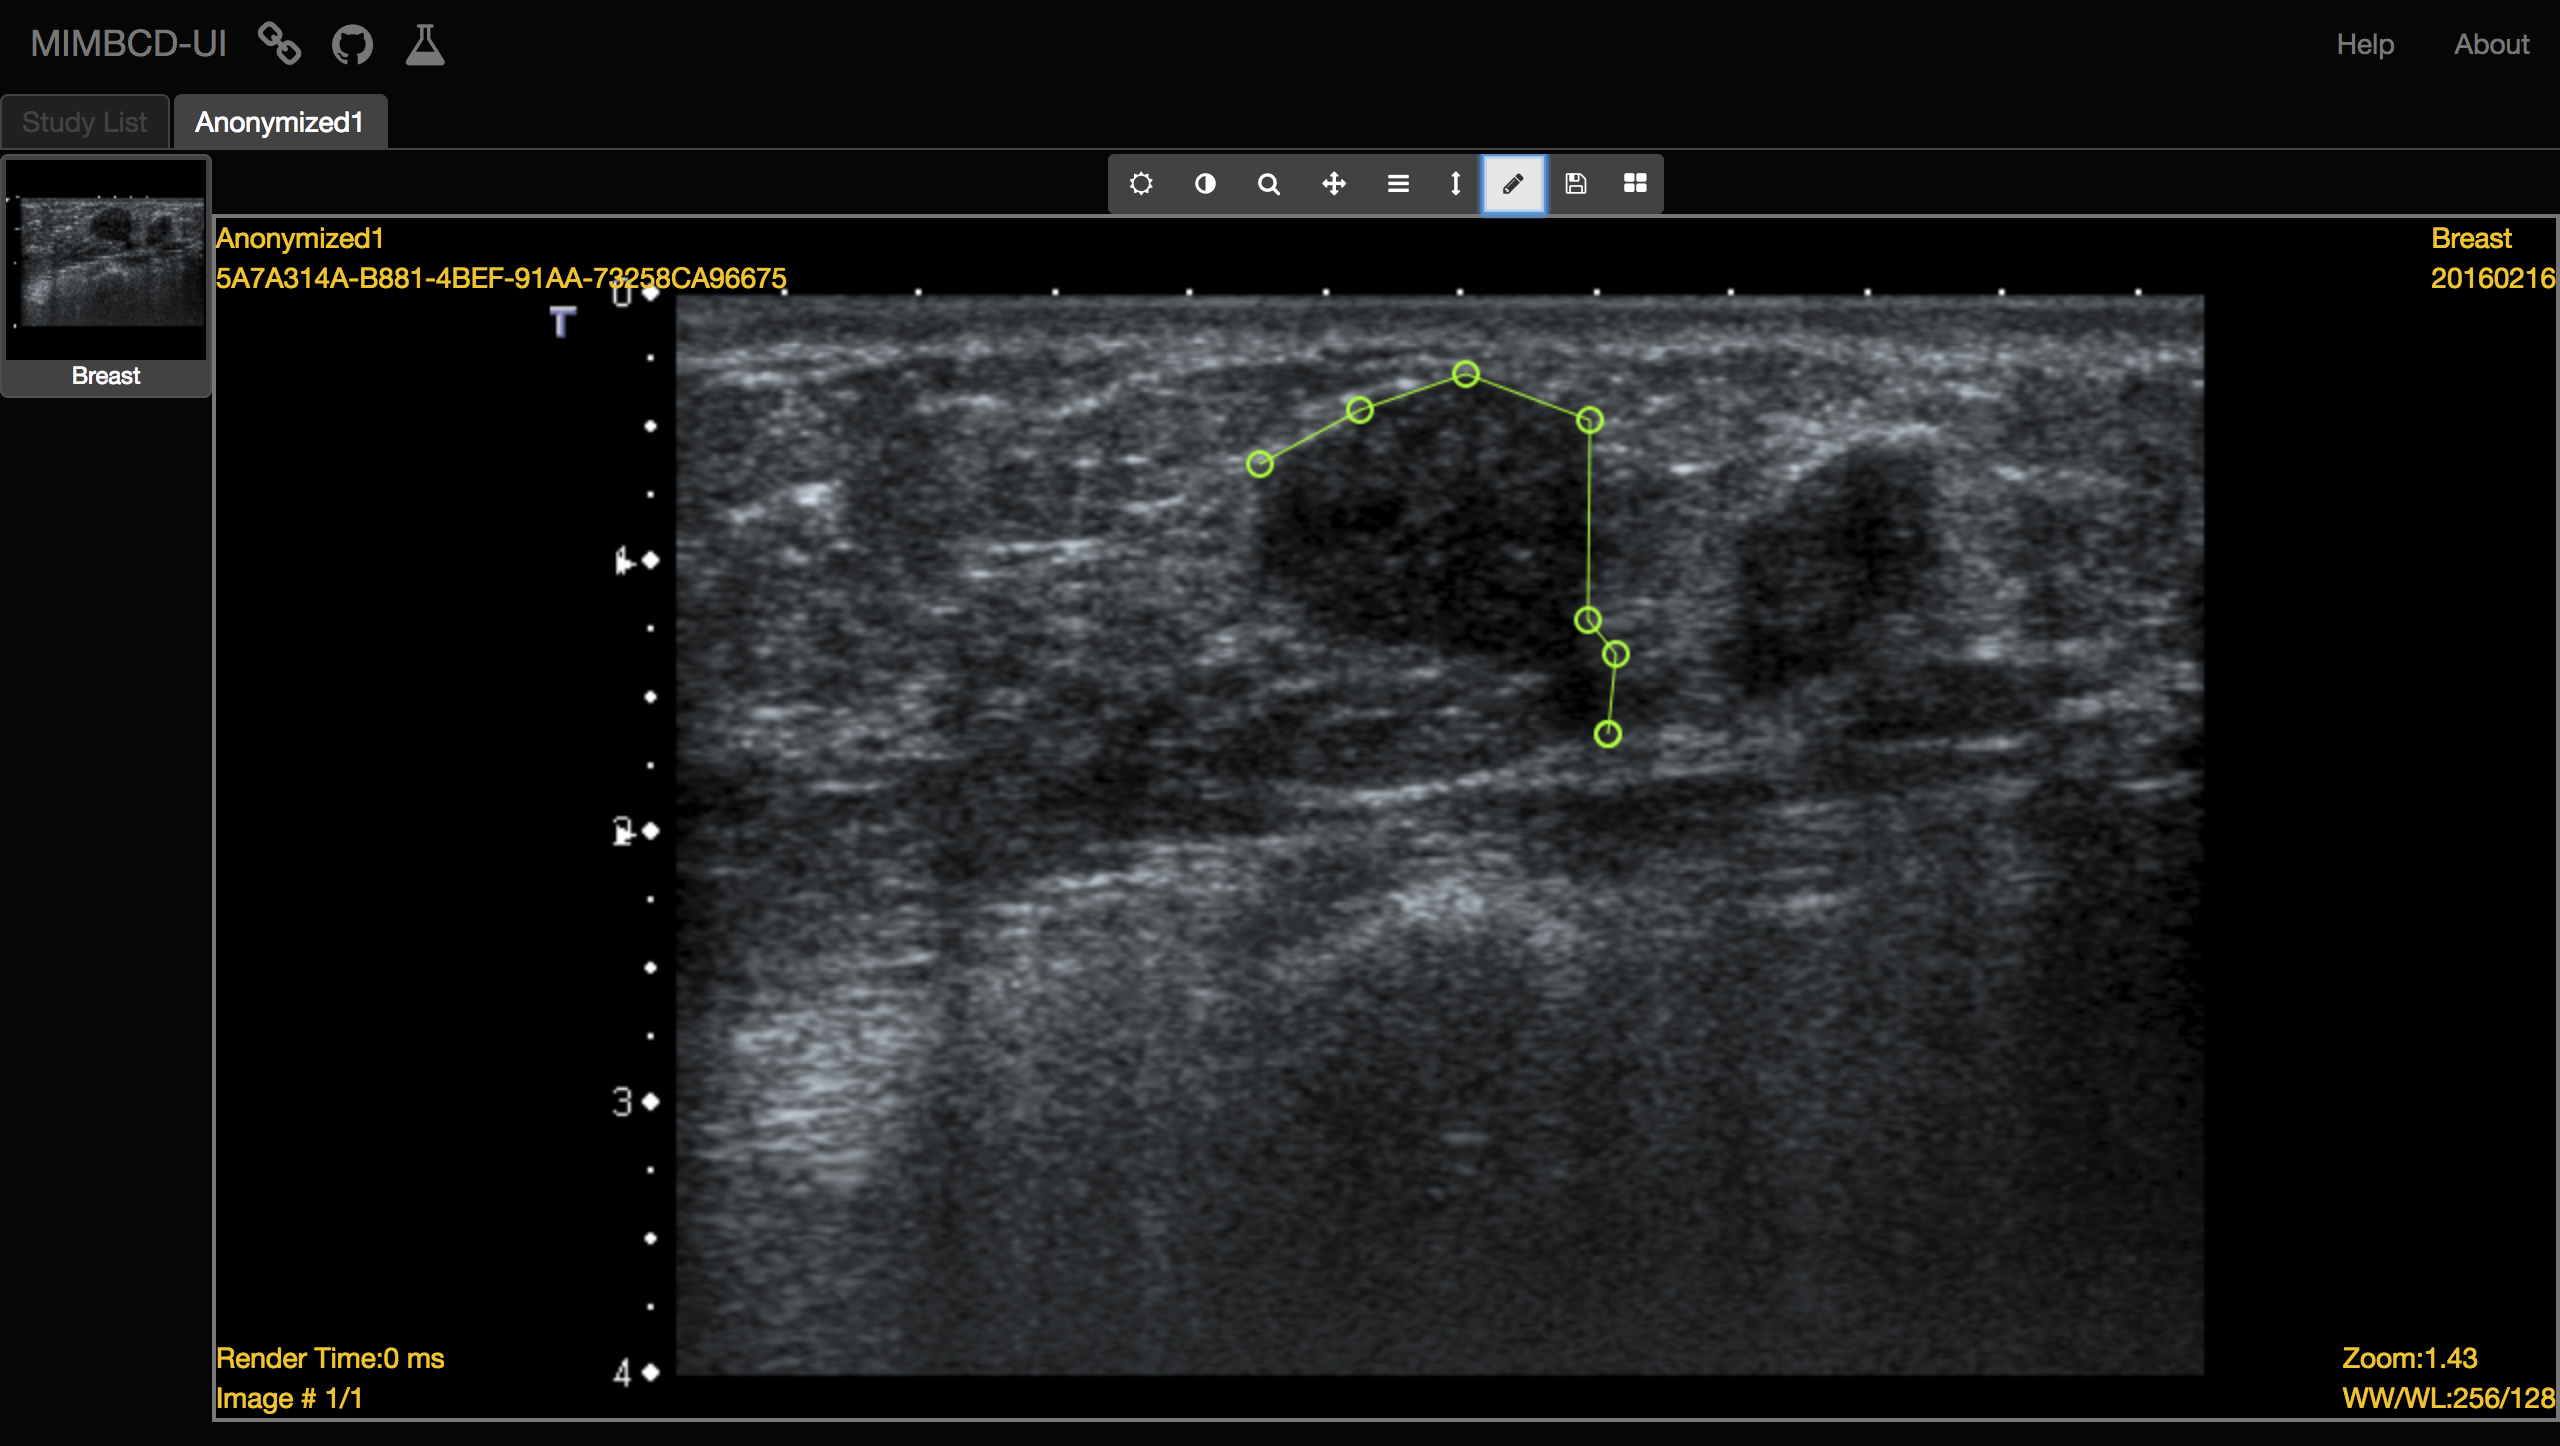
\includegraphics[width=0.75\textwidth]{graphics/anon1_annotations_start.png}
\end{center}

\item Finish annotation by clicking on the first one;

\begin{center}
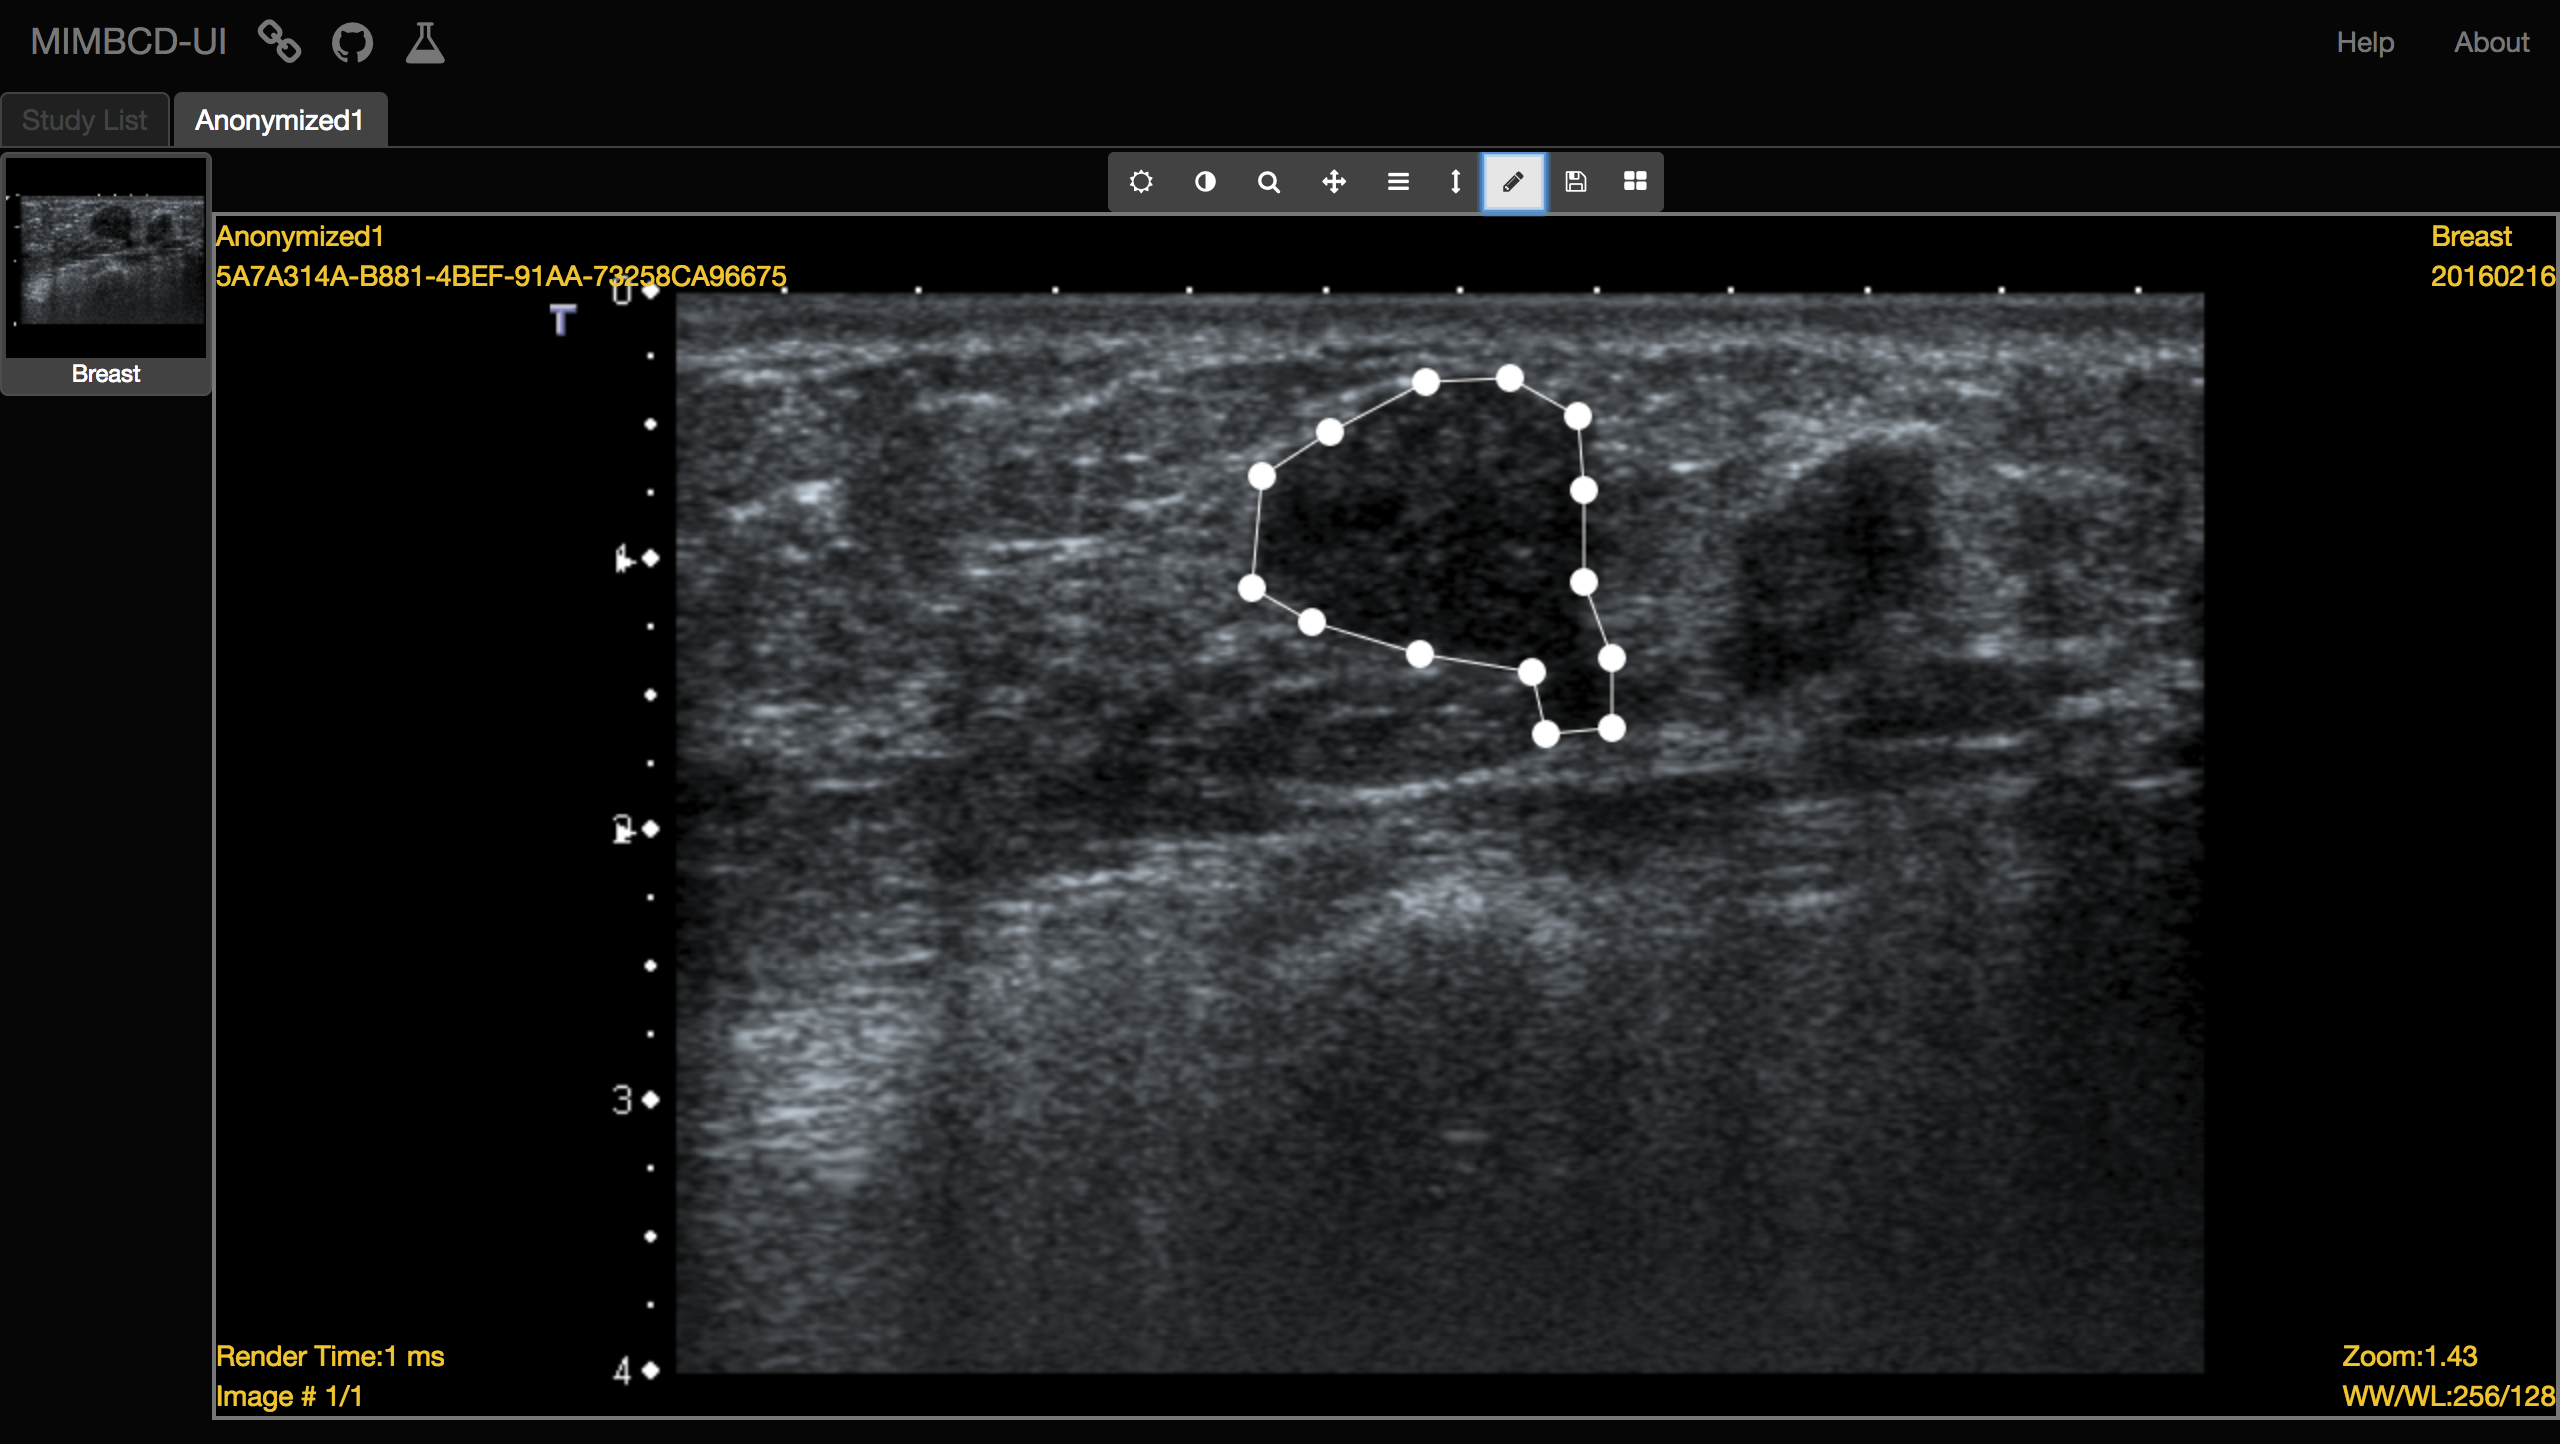
\includegraphics[width=0.75\textwidth]{graphics/anon1_annotations_finish.png}
\end{center}

\end{enumerate}

\bibliography{bibliography.bib}

\printindex

\end{document}
